\documentclass[11pt]{article}

\usepackage{amsmath}
\usepackage{amsmath}
\usepackage{amssymb}
\usepackage{mathtools,bbm}

\usepackage{comment}

\usepackage{micahcorah}

\usepackage{tikz}
\usepackage{pgfplots}
\usepackage{pgfplotstable}
\usetikzlibrary{arrows.meta}
\usetikzlibrary{backgrounds}

\usepackage{subcaption}
\usepackage{caption}

\captionsetup{font=footnotesize,compatibility=false,labelfont=bf}
\captionsetup[subfigure]{font=footnotesize,labelfont=bf}

\usepackage{graphicx}
\graphicspath{{./figures/}}

\usepackage[
hidelinks,
breaklinks,
colorlinks,
linkcolor=black,
citecolor=black,
filecolor=red,
urlcolor=blue
]{hyperref}

\usepackage[numbers]{natbib}

\showdevelopmenttrue

%%%%%%%%%%%%%%%%%%%%%%%%%%%%%%%%%%%%%%%%%%%%%%%%%%%%%%%%%%%%%%%%%%%%%%%%%
\pagestyle{plain}                                                      %%
%%%%%%%%%% EXACT 1in MARGINS %%%%%%%                                   %%
\setlength{\textwidth}{6.5in}     %%                                   %%
\setlength{\oddsidemargin}{0in}   %% (It is recommended that you       %%
\setlength{\evensidemargin}{0in}  %%  not change these parameters,     %%
\setlength{\textheight}{8.5in}    %%  at the risk of having your       %%
\setlength{\topmargin}{0in}       %%  proposal dismissed on the basis  %%
\setlength{\headheight}{0in}      %%  of incorrect formatting!!!)      %%
\setlength{\headsep}{0in}         %%                                   %%
\setlength{\footskip}{.5in}       %%                                   %%
%%%%%%%%%%%%%%%%%%%%%%%%%%%%%%%%%%%%                                   %%
% \bibliographystyle{plain}                                            %%
%%%%%%%%%%%%%%%%%%%%%%%%%%%%%%%%%%%%%%%%%%%%%%%%%%%%%%%%%%%%%%%%%%%%%%%%%

% Fakesection: Front matter
\title{Large Scale Markerless Capture of Multiple Subjects
with Coordinated Cameras}
\author{Micah Corah (\texttt{micah.corah@mines.edu})
  \\
  Computer Science Department,
  Colorado School of Mines
}
\date{}

%%%%%%%%%%%%%%%%%%%%%%%%%%%%%%%%%%%%%%%%%%%%%%%%%%%%%%%%%%%%%%%%%%%%%%%%%%%%
%%%%%%%%%%%%%%%%%%%%%%% Document
%%%%%%%%%%%%%%%%%%%%%%%%%%%%%%%%%%%%%%%%%%%%%%%%%%%%%%%%%%%%%%%%%%%%%%%%%%%%
\begin{document}
\maketitle

\section{Abstract}

% concise summary of objectives methodology, and expected outcomes

The advent of technologies such as Gaussian Splatting promise a future where
large static and dynamic scenes can routinely be captured and reconstructed for
the purpose of photorealistic rendering or for analysis of biomechanics and
motion.
However, current methods for motion capture involve installing large
arrays of cameras to cover limited capture volumes.
Instead, we propose development of methods for low-cost, high-capture-volume
markerless motion capture based controlling fewer cameras
(such as pan-tilt-zoom units) to densely cover relevant parts of a dynamic
scene.
Our methods will enable tracking and capture of multiple subjects moving about a
large space such as a soccer field or a running track.
To do so, we will leverage methods we have recently developed for coordinating
multiple cameras to observe dynamic scenes---methods that enable coverage of
groups of subjects as they move together or apart or reorganize over the
duration of a task.
The proposed approach will be evaluated in laboratory and field environments via
comparison with static marker-based and markerless motion capture.
We plan to release key components of the system as open-source software and will
publish results in premier robotics conferences.

\paragraph{Primary keyword:}
\emph{Capture Planning for Large 3D Spaces}

\section{Introduction}

\subsection{Problem \& Objective}

Existing markerless motion capture systems rely on collections of static cameras
to reconstruct human motion in a capture volume.
As a result, capturing motion of groups of people moving over large spaces and
in situ becomes prohibitively challenging due to requirements for increasing
amounts of cameras and infrastructure to cover the intended capture volume.
With this proposal, we seek to integrate methods of autonomous camera control
for filming multiple subjects and multi-camera methods for markerless motion
capture to enable motion capture in large spaces and with multiple subjects via
systems consisting of multiple pan-tilt-zoom cameras.

\begin{figure}
  \centering
  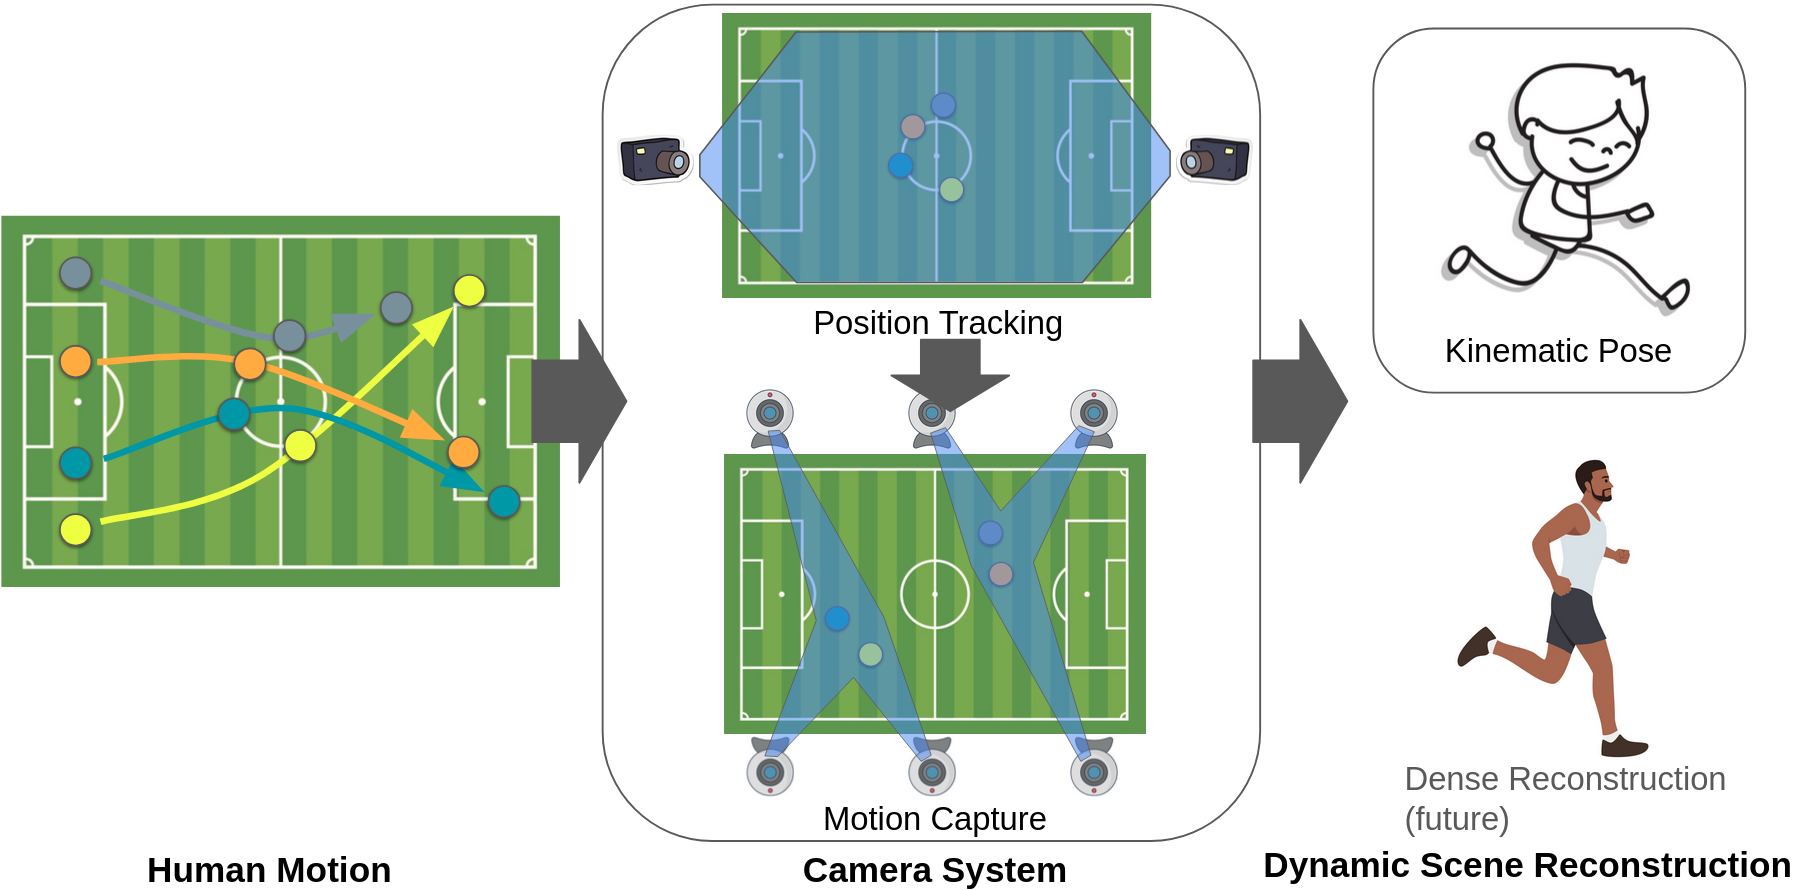
\includegraphics[width=0.9\linewidth]{figures/PTZ_Motion_Capture_Diagram.png}
  \caption{Graphical illustration of the proposed approach to
    markerless motion capture with multiple tracked subjects based on a
    robotic multi-camera system consisting of a small number of pan-tilt-zoom
    cameras.
    \emph{During the timeline of the proposed work, we expect to focus on
    kinematic reconstruction of skeletal human motion.}
    However, we expect our methods to be equally relevant to dense
    reconstruction via developing methods such as Gaussian splatting.
  }%
  \label{fig:markerless_system}
\end{figure}

% Background (state of art), significance, gap, impact
\subsection{Background \& Significance}

Over the past five years, markerless motion capture has transitioned from
research topic to product, and software and hardware offerings have emerged,
often from leading companies in the marker-based space e.g., Vicon, Optitrack,
or Qualisys.
One of the goals of this project will be to spur development of low-cost motion
capture systems that can be readily installed at and serve sports facilities and
arenas.
% Could add more detail here on biomechanics data collection
These systems promise applications varying from walk-in virtual reality
worlds\footnote{%
  Vicon demo ``Clockwork Forest'' presented at SIGGRAPH 2023:
  \url{https://www.youtube.com/watch?v=3Ex4XwBqvjA}
}
to the ability to collect biomechanics data for medical evaluations with minimal
time and preparation~\citep{wade2022peerj}.
Yet, like their marker-based cousins, these systems consist of large numbers of
cameras (e.g. 8+) that must be carefully placed and mounted to tripods or a
truss system and rigorously calibrated.

The research community meanwhile has sought to cast away the anchor of
fixed infrastructure by developing markerless motion capture capabilities around
formations of UAVs~\citep{saini2019iccv,ho2021iros,hong2024eccv,saini2022ral}.
While these aerial systems would not promise accuracy comparable to systems
built around fixed cameras with calibrated extrinsics, they instead promise the
ability to reconstruct human motion outdoors and largely without bounds.
These systems have another, less obvious, limitation: research on aerial
markerless motion capture has largely focused on reconstructing motion of
individual people.
Further, because these approaches generally rely on robots that fly in a
circular formation around one subject, capturing multiple subjects, especially
if those subjects may sometimes move apart, poses a significant challenge
regarding view planning and coordination.

Rather than controlling the locations of the cameras to follow the subject or
subjects, we may consider directing the fields-of-view of a small number of
fixed cameras to similarly observe and reconstruct motions of the subjects as
they move about a large capture volume.
In fact, markerless motion capture with pan-tilt-zoom (PTZ) cameras at fixed
locations but with uncertain orientations has been studied along with
application to downhill skiing~\citep{bachmann20193dv}.
Yet, there has been little interest overall in developing markerless motion
capture systems based on PTZ cameras and that is despite use of gimbal cameras
with aerial systems.
Moreover, neither body of work addresses the general problem of controlling
viewpoints and zoom for multiple cameras, especially as subjects may move apart
and come back together again.

\subsection{Challenges}

\begin{itemize}
  \item Distributing camera views over subjects and obtain observations from
    multiple perspectives
  \item Coverage of multiple subjects and groups that may spread out or
    rearrange
  \item Identifying and tracking subjects for motion capture and predicting
    their motion
  \item Uncertainty in intrinsics and extrinsics
  \item Achieving adequate coverage and detail for the desired reconstruction
    task
\end{itemize}

\subsection{Impacts}

The most direct benefit to Samsung will be contribution toward development of a
new technology product market in the sector of professional and amateur sports
where Samsung already has a strong presence.
This project is also relevant to the interests of Samsung Research America.
% Digital humans (in situ data collection)
% Transfer learning (humanoid robots.
% VR
Primarily, proposed methods will enable development of human motion capture
datasets that feature greater diversity of movement, interactions between
multiple subjects, and minimally invasive methods.
This will come about via enabling in situ markerless motion capture data
collection in domains where doing so would otherwise be challenging or
infeasible due to the scale of the capture volume.
This particularly applies to individual and team sports but may also reduce
barriers to collect motion capture data for dance and other sorts of
performance.
This data will elevate SRA's work on Digital Humans by enabling training of
neural network models that improve reconstruction quality and behavior
generation.
Likewise, this data may have similar impacts improving AR and VR systems.
Moreover, in combination with Gaussian splatting or neural fields methods, the
work we propose could enable development of VR applications for professional
sports media.


\section{Gap in state-of-art and contribution}

\begin{itemize}
  \item Permanent and semi-permanent installations based on large numbers of
    cameras
  \item Aerial motion capture systems:
    limited to small number of subjects, battery life and safety challenges,
    formations and limited camera coordination;
    \emph{Demonstrating plausibility of of reconstruction with uncalibrated or
    uncertain extrinsics}
  \item Datasets and camera motion: scale and uncertain intrinsics?
\end{itemize}

\subsection{Contributions}

\section{Methods}

We propose developing a markerless motion capture system based on a small number
of pan tilt zoom cameras (e.g. 4--8) that can autonomously track multiple
subjects moving together and separately over a large space such as a football
field or running track.
A key part of this approach will involve integration of assignment-free view
planning methods we have developed for this multi-camera, multi-subject setting
based on submodular optimization methods~\citep{suresh2024iros,hughes2024cdc}.

\subsection{Multi-camera coordination}

Autonomous camera view planning is a key element of our approach.
Our prior works on this topic present methods to optimize and maximize pixel
densities over subjects' surfaces for multiple cameras
jointly~\citep{suresh2024iros,hughes2024cdc}.
This approach applies submodular optimization methods to maximize view quality
directly without relying on fixed assignments and guaranteeing constant-factor
suboptimality for approximate solutions to the joint optimization problem.
Simulation results involving a team of UAVs filming multiple moving subjects
demonstrated emergent assignment and formation behaviors and superior
performance compared to formation methods when subjects split and rejoin
(Fig.~\ref{fig:qualitative}).
We propose applying a similar approach to planning for pan-tilt-zoom cameras by
reformulating the earlier planning problem according to the PTZ configuration
space.

\subsection{Reconstruction}

Having developed a camera controller that autonomously obtains views of subjects
from multiple perspectives, we plan to adopt similar methods for skeletal
reconstruction and markerless motion capture as have been demonstrated
previously for systems consisting of multiple PTZ
cameras~\citep{bachmann20193dv} or
UAVs~\citep{saini2019iccv,ho2021iros,hong2024eccv,saini2022ral}.

\subsection{Systems and experimental validation}

\begin{itemize}
  \item Laboratory experiments combining marker-based and markerless evaluation
    with static calibrated cameras will serve to validate the approach in the
    first phase
  \item The second phase will consist of evaluation via field experiments at an
    outdoor field on the university campus.
    Metric accuracy will be validated by surveying keypoints in the capture
    volume and collecting datasets consisting of motion through those keypoints
  \item Low-cost markerless capture (FreeMoCap) in lab and field
\end{itemize}

\section{Goals and Milestones}

% Timeline with milestones and deliverables
\begin{itemize}
  \item (Aug--Oct '26) Prototype multi-camera view planning in indoor
    laboratory environment
  \item (Nov '26--Jan '27) Prototype 3D skeletal reconstruction based on
    pan-tilt-zoom camera streams
  \item (Feb '27) Perform comparative experiments for skeletal reconstruction in
    laboratory environment
  \item (Feb '27) \textbf{Milestone:} submit paper based on initial system and
    experiments to IROS'27
  \item (March--April '27) Develop and evaluate person-tracking system for large
    environment based on flat ground assumption
  \item (May '27) Integrate updated tracking system; develop systems and
    procedures for large scale outdoor experiments
  \item (June '27) Perform experiments on outdoor fields
  \item (July--Aug '27) \textbf{Milestone:}
    Write paper based on field experiments for submission to ICRA'28
\end{itemize}

% Research plan and technical approach (methodology, analysis techniques,
% validation)

\begin{figure*}
\centering
\setlength{\tabcolsep}{1pt}
\setlength{\figureheight}{1.2in}
      \resizebox{\linewidth}{!}{
      \begin{tikzpicture}[x=0.75pt,y=0.75pt,yscale=-1,xscale=1]
%uncomment if require: \path (0,356); %set diagram left start at 0, and has height of 356

%Image [id:dp7277736187599475] 
\draw (330.19,269.48) node  {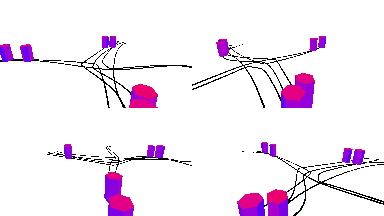
\includegraphics[width=134.71pt,height=75.77pt]{res_0020.png}};
%Shape: Rectangle [id:dp9098908258042562] 
\draw   (240.39,218.97) -- (420,218.97) -- (420,319.63) -- (240.39,319.63) -- cycle ;
%Straight Lines [id:da5638926407429237] 
\draw    (330.19,218.97) -- (330.19,319.63) ;
%Straight Lines [id:da8403080327763022] 
\draw    (240,269.3) -- (419.52,269.3) ;


%Shape: Grid [id:dp8720285301043298] 
\draw  [draw opacity=0][line width=0.75]  (861.64,33.44) -- (1001.64,33.44) -- (1001.64,173.44) -- (861.64,173.44) -- cycle ; \draw  [color={rgb, 255:red, 0; green, 0; blue, 0 }  ,draw opacity=0.06 ][line width=0.75]  (866.64,33.44) -- (866.64,173.44)(871.64,33.44) -- (871.64,173.44)(876.64,33.44) -- (876.64,173.44)(881.64,33.44) -- (881.64,173.44)(886.64,33.44) -- (886.64,173.44)(891.64,33.44) -- (891.64,173.44)(896.64,33.44) -- (896.64,173.44)(901.64,33.44) -- (901.64,173.44)(906.64,33.44) -- (906.64,173.44)(911.64,33.44) -- (911.64,173.44)(916.64,33.44) -- (916.64,173.44)(921.64,33.44) -- (921.64,173.44)(926.64,33.44) -- (926.64,173.44)(931.64,33.44) -- (931.64,173.44)(936.64,33.44) -- (936.64,173.44)(941.64,33.44) -- (941.64,173.44)(946.64,33.44) -- (946.64,173.44)(951.64,33.44) -- (951.64,173.44)(956.64,33.44) -- (956.64,173.44)(961.64,33.44) -- (961.64,173.44)(966.64,33.44) -- (966.64,173.44)(971.64,33.44) -- (971.64,173.44)(976.64,33.44) -- (976.64,173.44)(981.64,33.44) -- (981.64,173.44)(986.64,33.44) -- (986.64,173.44)(991.64,33.44) -- (991.64,173.44)(996.64,33.44) -- (996.64,173.44) ; \draw  [color={rgb, 255:red, 0; green, 0; blue, 0 }  ,draw opacity=0.06 ][line width=0.75]  (861.64,38.44) -- (1001.64,38.44)(861.64,43.44) -- (1001.64,43.44)(861.64,48.44) -- (1001.64,48.44)(861.64,53.44) -- (1001.64,53.44)(861.64,58.44) -- (1001.64,58.44)(861.64,63.44) -- (1001.64,63.44)(861.64,68.44) -- (1001.64,68.44)(861.64,73.44) -- (1001.64,73.44)(861.64,78.44) -- (1001.64,78.44)(861.64,83.44) -- (1001.64,83.44)(861.64,88.44) -- (1001.64,88.44)(861.64,93.44) -- (1001.64,93.44)(861.64,98.44) -- (1001.64,98.44)(861.64,103.44) -- (1001.64,103.44)(861.64,108.44) -- (1001.64,108.44)(861.64,113.44) -- (1001.64,113.44)(861.64,118.44) -- (1001.64,118.44)(861.64,123.44) -- (1001.64,123.44)(861.64,128.44) -- (1001.64,128.44)(861.64,133.44) -- (1001.64,133.44)(861.64,138.44) -- (1001.64,138.44)(861.64,143.44) -- (1001.64,143.44)(861.64,148.44) -- (1001.64,148.44)(861.64,153.44) -- (1001.64,153.44)(861.64,158.44) -- (1001.64,158.44)(861.64,163.44) -- (1001.64,163.44)(861.64,168.44) -- (1001.64,168.44) ; \draw  [color={rgb, 255:red, 0; green, 0; blue, 0 }  ,draw opacity=0.06 ][line width=0.75]  (861.64,33.44) -- (1001.64,33.44) -- (1001.64,173.44) -- (861.64,173.44) -- cycle ;
%Flowchart: Process [id:dp7692999741250126] 
\draw  [fill={rgb, 255:red, 0; green, 0; blue, 0 }  ,fill opacity=0.23 ] (950.2,148.26) -- (953.87,148.26) -- (953.87,151.84) -- (950.2,151.84) -- cycle ;
%Straight Lines [id:da8280615441828281] 
\draw    (953.87,148.26) -- (955.44,146.53) ;
%Shape: Ellipse [id:dp2732921033119995] 
\draw   (953.49,146.53) .. controls (953.49,145.45) and (954.36,144.58) .. (955.44,144.58) .. controls (956.52,144.58) and (957.39,145.45) .. (957.39,146.53) .. controls (957.39,147.61) and (956.52,148.48) .. (955.44,148.48) .. controls (954.36,148.48) and (953.49,147.61) .. (953.49,146.53) -- cycle ;
%Straight Lines [id:da3486019145641228] 
\draw    (953.84,151.76) -- (955.5,153.4) ;
%Shape: Ellipse [id:dp33583143781746005] 
\draw   (955.58,151.45) .. controls (956.66,151.5) and (957.5,152.41) .. (957.45,153.49) .. controls (957.4,154.57) and (956.49,155.41) .. (955.41,155.36) .. controls (954.33,155.31) and (953.49,154.4) .. (953.54,153.32) .. controls (953.59,152.24) and (954.5,151.4) .. (955.58,151.45) -- cycle ;
%Straight Lines [id:da32277028188015144] 
\draw    (950.13,148.31) -- (948.54,146.59) ;
%Shape: Ellipse [id:dp15733291912856218] 
\draw   (950.52,146.59) .. controls (950.52,145.51) and (949.63,144.63) .. (948.54,144.63) .. controls (947.44,144.63) and (946.55,145.51) .. (946.55,146.59) .. controls (946.55,147.67) and (947.44,148.54) .. (948.54,148.54) .. controls (949.63,148.54) and (950.52,147.67) .. (950.52,146.59) -- cycle ;
%Straight Lines [id:da3318354105958701] 
\draw    (950.16,151.82) -- (948.48,153.46) ;
%Shape: Ellipse [id:dp264824062350145] 
\draw   (948.39,151.51) .. controls (947.3,151.56) and (946.45,152.47) .. (946.5,153.55) .. controls (946.55,154.63) and (947.47,155.46) .. (948.57,155.41) .. controls (949.67,155.36) and (950.51,154.45) .. (950.46,153.37) .. controls (950.41,152.29) and (949.49,151.46) .. (948.39,151.51) -- cycle ;
%Shape: Arc [id:dp7234580380045712] 
\draw  [draw opacity=0][fill={rgb, 255:red, 250; green, 33; blue, 33 }  ,fill opacity=0.14 ] (925.92,121.36) .. controls (932.66,114.65) and (941.94,110.5) .. (952.2,110.5) .. controls (962.47,110.5) and (971.78,114.67) .. (978.52,121.4) -- (952.2,147.72) -- cycle ; \draw  [draw opacity=0] (925.92,121.36) .. controls (932.66,114.65) and (941.94,110.5) .. (952.2,110.5) .. controls (962.47,110.5) and (971.78,114.67) .. (978.52,121.4) ;  
%Straight Lines [id:da29004653178866135] 
\draw [draw opacity=0]   (925.92,121.36) -- (952.1,148.34) ;
%Straight Lines [id:da4026425575850259] 
\draw [draw opacity=0]   (952.1,148.34) -- (978.52,121.4) ;

%Flowchart: Process [id:dp9746762046165662] 
\draw  [fill={rgb, 255:red, 0; green, 0; blue, 0 }  ,fill opacity=0.23 ] (986.82,110.47) -- (986.82,106.79) -- (990.4,106.79) -- (990.4,110.47) -- cycle ;
%Straight Lines [id:da6819852972538718] 
\draw    (986.82,106.79) -- (985.09,105.23) ;
%Shape: Ellipse [id:dp3810204521729641] 
\draw   (985.09,107.18) .. controls (984.01,107.18) and (983.14,106.31) .. (983.14,105.23) .. controls (983.14,104.15) and (984.01,103.27) .. (985.09,103.27) .. controls (986.17,103.27) and (987.04,104.15) .. (987.04,105.23) .. controls (987.04,106.31) and (986.17,107.18) .. (985.09,107.18) -- cycle ;
%Straight Lines [id:da6206870460758294] 
\draw    (990.32,106.83) -- (991.96,105.17) ;
%Shape: Ellipse [id:dp8743457946594126] 
\draw   (990.01,105.08) .. controls (990.06,104.01) and (990.97,103.17) .. (992.05,103.22) .. controls (993.13,103.27) and (993.97,104.18) .. (993.92,105.26) .. controls (993.87,106.34) and (992.95,107.17) .. (991.88,107.12) .. controls (990.8,107.08) and (989.96,106.16) .. (990.01,105.08) -- cycle ;
%Straight Lines [id:da7262536254049345] 
\draw    (986.87,110.54) -- (985.15,112.13) ;
%Shape: Ellipse [id:dp3218819146714573] 
\draw   (985.15,110.14) .. controls (984.07,110.14) and (983.19,111.03) .. (983.19,112.13) .. controls (983.19,113.23) and (984.07,114.12) .. (985.15,114.12) .. controls (986.22,114.12) and (987.1,113.23) .. (987.1,112.13) .. controls (987.1,111.03) and (986.22,110.14) .. (985.15,110.14) -- cycle ;
%Straight Lines [id:da6538232923150589] 
\draw    (990.38,110.51) -- (992.02,112.19) ;
%Shape: Ellipse [id:dp8734177549451376] 
\draw   (990.07,112.28) .. controls (990.12,113.37) and (991.03,114.22) .. (992.11,114.17) .. controls (993.19,114.12) and (994.02,113.19) .. (993.97,112.1) .. controls (993.92,111) and (993.01,110.15) .. (991.93,110.2) .. controls (990.85,110.25) and (990.02,111.18) .. (990.07,112.28) -- cycle ;
%Shape: Arc [id:dp3449046764056387] 
\draw  [draw opacity=0][fill={rgb, 255:red, 250; green, 33; blue, 33 }  ,fill opacity=0.14 ] (959.92,134.74) .. controls (953.21,128.01) and (949.06,118.72) .. (949.06,108.47) .. controls (949.06,98.19) and (953.23,88.89) .. (959.96,82.15) -- (986.28,108.47) -- cycle ; \draw  [draw opacity=0] (959.92,134.74) .. controls (953.21,128.01) and (949.06,118.72) .. (949.06,108.47) .. controls (949.06,98.19) and (953.23,88.89) .. (959.96,82.15) ;  
%Straight Lines [id:da6299838007348599] 
\draw [draw opacity=0]   (959.92,134.74) -- (986.9,108.57) ;
%Straight Lines [id:da6701985982352596] 
\draw [draw opacity=0]   (986.9,108.57) -- (959.96,82.15) ;

%Flowchart: Process [id:dp5056972909462676] 
\draw  [fill={rgb, 255:red, 0; green, 0; blue, 0 }  ,fill opacity=0.23 ] (938.2,58.68) -- (934.52,58.68) -- (934.52,55.1) -- (938.2,55.1) -- cycle ;
%Straight Lines [id:da6714788558111089] 
\draw    (934.52,58.68) -- (932.95,60.41) ;
%Shape: Ellipse [id:dp45435564162445075] 
\draw   (934.91,60.41) .. controls (934.91,61.49) and (934.03,62.36) .. (932.95,62.36) .. controls (931.87,62.36) and (931,61.49) .. (931,60.41) .. controls (931,59.33) and (931.87,58.46) .. (932.95,58.46) .. controls (934.03,58.46) and (934.91,59.33) .. (934.91,60.41) -- cycle ;
%Straight Lines [id:da05431220788460012] 
\draw    (934.55,55.18) -- (932.9,53.54) ;
%Shape: Ellipse [id:dp0028246012786978802] 
\draw   (932.81,55.49) .. controls (931.73,55.44) and (930.9,54.53) .. (930.95,53.45) .. controls (930.99,52.37) and (931.91,51.53) .. (932.99,51.58) .. controls (934.06,51.63) and (934.9,52.55) .. (934.85,53.62) .. controls (934.8,54.7) and (933.89,55.54) .. (932.81,55.49) -- cycle ;
%Straight Lines [id:da1085838184560246] 
\draw    (938.27,58.63) -- (939.86,60.35) ;
%Shape: Ellipse [id:dp8190356245493642] 
\draw   (937.87,60.35) .. controls (937.87,61.43) and (938.76,62.31) .. (939.86,62.31) .. controls (940.95,62.31) and (941.84,61.43) .. (941.84,60.35) .. controls (941.84,59.28) and (940.95,58.4) .. (939.86,58.4) .. controls (938.76,58.4) and (937.87,59.28) .. (937.87,60.35) -- cycle ;
%Straight Lines [id:da5115324596769721] 
\draw    (938.23,55.12) -- (939.91,53.48) ;
%Shape: Ellipse [id:dp6726775166664924] 
\draw   (940,55.43) .. controls (941.1,55.38) and (941.95,54.47) .. (941.9,53.39) .. controls (941.85,52.31) and (940.92,51.48) .. (939.82,51.53) .. controls (938.73,51.58) and (937.88,52.49) .. (937.93,53.57) .. controls (937.98,54.65) and (938.91,55.48) .. (940,55.43) -- cycle ;
%Shape: Arc [id:dp022551318169735435] 
\draw  [draw opacity=0][fill={rgb, 255:red, 250; green, 33; blue, 33 }  ,fill opacity=0.14 ] (962.47,85.58) .. controls (955.74,92.29) and (946.45,96.44) .. (936.2,96.44) .. controls (925.92,96.44) and (916.61,92.27) .. (909.88,85.54) -- (936.2,59.22) -- cycle ; \draw  [draw opacity=0] (962.47,85.58) .. controls (955.74,92.29) and (946.45,96.44) .. (936.2,96.44) .. controls (925.92,96.44) and (916.61,92.27) .. (909.88,85.54) ;  
%Straight Lines [id:da3771365627129253] 
\draw [draw opacity=0]   (962.47,85.58) -- (936.3,58.6) ;
%Straight Lines [id:da8711477193470645] 
\draw [draw opacity=0]   (936.3,58.6) -- (909.88,85.54) ;

%Flowchart: Process [id:dp32980237070801177] 
\draw  [fill={rgb, 255:red, 0; green, 0; blue, 0 }  ,fill opacity=0.23 ] (892.08,86.64) -- (892.08,90.31) -- (888.49,90.31) -- (888.49,86.64) -- cycle ;
%Straight Lines [id:da5741819102641925] 
\draw    (892.08,90.31) -- (893.8,91.88) ;
%Shape: Ellipse [id:dp5483421436224314] 
\draw   (893.8,89.93) .. controls (894.88,89.93) and (895.76,90.8) .. (895.76,91.88) .. controls (895.76,92.96) and (894.88,93.83) .. (893.8,93.83) .. controls (892.72,93.83) and (891.85,92.96) .. (891.85,91.88) .. controls (891.85,90.8) and (892.72,89.93) .. (893.8,89.93) -- cycle ;
%Straight Lines [id:da03947151663204962] 
\draw    (888.57,90.28) -- (886.93,91.94) ;
%Shape: Ellipse [id:dp09715063806736679] 
\draw   (888.88,92.02) .. controls (888.83,93.1) and (887.92,93.94) .. (886.84,93.89) .. controls (885.76,93.84) and (884.93,92.93) .. (884.98,91.85) .. controls (885.02,90.77) and (885.94,89.93) .. (887.02,89.98) .. controls (888.09,90.03) and (888.93,90.95) .. (888.88,92.02) -- cycle ;
%Straight Lines [id:da7122474483071757] 
\draw    (892.02,86.57) -- (893.75,84.98) ;
%Shape: Ellipse [id:dp9895912799375546] 
\draw   (893.75,86.96) .. controls (894.83,86.96) and (895.7,86.07) .. (895.7,84.98) .. controls (895.7,83.88) and (894.83,82.99) .. (893.75,82.99) .. controls (892.67,82.99) and (891.79,83.88) .. (891.79,84.98) .. controls (891.79,86.07) and (892.67,86.96) .. (893.75,86.96) -- cycle ;
%Straight Lines [id:da7024538483604319] 
\draw    (888.51,86.6) -- (886.87,84.92) ;
%Shape: Ellipse [id:dp13551883967126965] 
\draw   (888.82,84.83) .. controls (888.78,83.74) and (887.86,82.89) .. (886.78,82.94) .. controls (885.71,82.99) and (884.87,83.91) .. (884.92,85.01) .. controls (884.97,86.11) and (885.88,86.95) .. (886.96,86.9) .. controls (888.04,86.85) and (888.87,85.93) .. (888.82,84.83) -- cycle ;
%Shape: Arc [id:dp2881030853096158] 
\draw  [draw opacity=0][fill={rgb, 255:red, 250; green, 33; blue, 33 }  ,fill opacity=0.14 ] (918.98,62.36) .. controls (925.69,69.1) and (929.83,78.38) .. (929.83,88.64) .. controls (929.83,98.91) and (925.67,108.22) .. (918.93,114.96) -- (892.61,88.64) -- cycle ; \draw  [draw opacity=0] (918.98,62.36) .. controls (925.69,69.1) and (929.83,78.38) .. (929.83,88.64) .. controls (929.83,98.91) and (925.67,108.22) .. (918.93,114.96) ;  
%Straight Lines [id:da9920625195513388] 
\draw [draw opacity=0]   (918.98,62.36) -- (891.99,88.54) ;
%Straight Lines [id:da9502857064133408] 
\draw [draw opacity=0]   (891.99,88.54) -- (918.93,114.96) ;

%Shape: Circle [id:dp4589607516571401] 
\draw  [draw opacity=0][fill={rgb, 255:red, 144; green, 19; blue, 254 }  ,fill opacity=1 ] (947.54,87.79) .. controls (947.54,85.39) and (949.49,83.44) .. (951.89,83.44) .. controls (954.29,83.44) and (956.24,85.39) .. (956.24,87.79) .. controls (956.24,90.2) and (954.29,92.14) .. (951.89,92.14) .. controls (949.49,92.14) and (947.54,90.2) .. (947.54,87.79) -- cycle ;
%Shape: Circle [id:dp002051093601916687] 
\draw  [draw opacity=0][fill={rgb, 255:red, 65; green, 117; blue, 5 }  ,fill opacity=1 ] (941.69,88.28) .. controls (941.69,85.87) and (943.64,83.93) .. (946.04,83.93) .. controls (948.44,83.93) and (950.39,85.87) .. (950.39,88.28) .. controls (950.39,90.68) and (948.44,92.63) .. (946.04,92.63) .. controls (943.64,92.63) and (941.69,90.68) .. (941.69,88.28) -- cycle ;
%Shape: Circle [id:dp04307192517239877] 
\draw  [draw opacity=0][fill={rgb, 255:red, 189; green, 16; blue, 224 }  ,fill opacity=1 ] (912.39,87.69) .. controls (912.39,85.29) and (914.34,83.34) .. (916.74,83.34) .. controls (919.14,83.34) and (921.09,85.29) .. (921.09,87.69) .. controls (921.09,90.1) and (919.14,92.04) .. (916.74,92.04) .. controls (914.34,92.04) and (912.39,90.1) .. (912.39,87.69) -- cycle ;
%Shape: Circle [id:dp2703519234007956] 
\draw  [draw opacity=0][fill={rgb, 255:red, 126; green, 211; blue, 33 }  ,fill opacity=1 ] (914.52,95.61) .. controls (914.52,93.21) and (916.47,91.26) .. (918.87,91.26) .. controls (921.27,91.26) and (923.22,93.21) .. (923.22,95.61) .. controls (923.22,98.01) and (921.27,99.96) .. (918.87,99.96) .. controls (916.47,99.96) and (914.52,98.01) .. (914.52,95.61) -- cycle ;
%Shape: Circle [id:dp4960485924059912] 
\draw  [draw opacity=0][fill={rgb, 255:red, 139; green, 87; blue, 42 }  ,fill opacity=1 ] (959.88,118.94) .. controls (959.88,116.53) and (961.84,114.57) .. (964.26,114.57) .. controls (966.68,114.57) and (968.64,116.53) .. (968.64,118.94) .. controls (968.64,121.36) and (966.68,123.32) .. (964.26,123.32) .. controls (961.84,123.32) and (959.88,121.36) .. (959.88,118.94) -- cycle ;
%Shape: Circle [id:dp49454859146933594] 
\draw  [draw opacity=0][fill={rgb, 255:red, 208; green, 2; blue, 27 }  ,fill opacity=1 ] (957.69,124.69) .. controls (957.69,122.29) and (959.64,120.34) .. (962.04,120.34) .. controls (964.44,120.34) and (966.39,122.29) .. (966.39,124.69) .. controls (966.39,127.1) and (964.44,129.04) .. (962.04,129.04) .. controls (959.64,129.04) and (957.69,127.1) .. (957.69,124.69) -- cycle ;

%Shape: Grid [id:dp9680513535880224] 
\draw  [draw opacity=0][line width=0.75]  (468.91,29) -- (608.91,29) -- (608.91,169) -- (468.91,169) -- cycle ; \draw  [color={rgb, 255:red, 0; green, 0; blue, 0 }  ,draw opacity=0.06 ][line width=0.75]  (473.91,29) -- (473.91,169)(478.91,29) -- (478.91,169)(483.91,29) -- (483.91,169)(488.91,29) -- (488.91,169)(493.91,29) -- (493.91,169)(498.91,29) -- (498.91,169)(503.91,29) -- (503.91,169)(508.91,29) -- (508.91,169)(513.91,29) -- (513.91,169)(518.91,29) -- (518.91,169)(523.91,29) -- (523.91,169)(528.91,29) -- (528.91,169)(533.91,29) -- (533.91,169)(538.91,29) -- (538.91,169)(543.91,29) -- (543.91,169)(548.91,29) -- (548.91,169)(553.91,29) -- (553.91,169)(558.91,29) -- (558.91,169)(563.91,29) -- (563.91,169)(568.91,29) -- (568.91,169)(573.91,29) -- (573.91,169)(578.91,29) -- (578.91,169)(583.91,29) -- (583.91,169)(588.91,29) -- (588.91,169)(593.91,29) -- (593.91,169)(598.91,29) -- (598.91,169)(603.91,29) -- (603.91,169) ; \draw  [color={rgb, 255:red, 0; green, 0; blue, 0 }  ,draw opacity=0.06 ][line width=0.75]  (468.91,34) -- (608.91,34)(468.91,39) -- (608.91,39)(468.91,44) -- (608.91,44)(468.91,49) -- (608.91,49)(468.91,54) -- (608.91,54)(468.91,59) -- (608.91,59)(468.91,64) -- (608.91,64)(468.91,69) -- (608.91,69)(468.91,74) -- (608.91,74)(468.91,79) -- (608.91,79)(468.91,84) -- (608.91,84)(468.91,89) -- (608.91,89)(468.91,94) -- (608.91,94)(468.91,99) -- (608.91,99)(468.91,104) -- (608.91,104)(468.91,109) -- (608.91,109)(468.91,114) -- (608.91,114)(468.91,119) -- (608.91,119)(468.91,124) -- (608.91,124)(468.91,129) -- (608.91,129)(468.91,134) -- (608.91,134)(468.91,139) -- (608.91,139)(468.91,144) -- (608.91,144)(468.91,149) -- (608.91,149)(468.91,154) -- (608.91,154)(468.91,159) -- (608.91,159)(468.91,164) -- (608.91,164) ; \draw  [color={rgb, 255:red, 0; green, 0; blue, 0 }  ,draw opacity=0.06 ][line width=0.75]  (468.91,29) -- (608.91,29) -- (608.91,169) -- (468.91,169) -- cycle ;
%Flowchart: Process [id:dp7337979330445772] 
\draw  [fill={rgb, 255:red, 0; green, 0; blue, 0 }  ,fill opacity=0.23 ] (521.89,152.73) -- (525.56,152.73) -- (525.56,156.31) -- (521.89,156.31) -- cycle ;
%Straight Lines [id:da9617359119677362] 
\draw    (525.56,152.73) -- (527.13,151) ;
%Shape: Ellipse [id:dp21575671193852086] 
\draw   (525.18,151) .. controls (525.18,149.92) and (526.05,149.05) .. (527.13,149.05) .. controls (528.21,149.05) and (529.08,149.92) .. (529.08,151) .. controls (529.08,152.08) and (528.21,152.96) .. (527.13,152.96) .. controls (526.05,152.96) and (525.18,152.08) .. (525.18,151) -- cycle ;
%Straight Lines [id:da27139860599258947] 
\draw    (525.53,156.24) -- (527.19,157.88) ;
%Shape: Ellipse [id:dp053283393329296214] 
\draw   (527.27,155.93) .. controls (528.35,155.97) and (529.19,156.89) .. (529.14,157.97) .. controls (529.09,159.04) and (528.18,159.88) .. (527.1,159.83) .. controls (526.02,159.78) and (525.18,158.87) .. (525.23,157.79) .. controls (525.28,156.71) and (526.2,155.88) .. (527.27,155.93) -- cycle ;
%Straight Lines [id:da04257717833372321] 
\draw    (521.82,152.79) -- (520.23,151.06) ;
%Shape: Ellipse [id:dp4364860546632132] 
\draw   (522.21,151.06) .. controls (522.21,149.98) and (521.32,149.11) .. (520.23,149.11) .. controls (519.13,149.11) and (518.24,149.98) .. (518.24,151.06) .. controls (518.24,152.14) and (519.13,153.01) .. (520.23,153.01) .. controls (521.32,153.01) and (522.21,152.14) .. (522.21,151.06) -- cycle ;
%Straight Lines [id:da6269442761049746] 
\draw    (521.85,156.29) -- (520.17,157.93) ;
%Shape: Ellipse [id:dp32500322020844163] 
\draw   (520.08,155.98) .. controls (518.99,156.03) and (518.14,156.94) .. (518.19,158.02) .. controls (518.24,159.1) and (519.16,159.93) .. (520.26,159.89) .. controls (521.36,159.84) and (522.2,158.92) .. (522.15,157.85) .. controls (522.1,156.77) and (521.18,155.93) .. (520.08,155.98) -- cycle ;
%Shape: Arc [id:dp665561479134849] 
\draw  [draw opacity=0][fill={rgb, 255:red, 250; green, 33; blue, 33 }  ,fill opacity=0.14 ] (497.61,125.83) .. controls (504.35,119.12) and (513.63,114.97) .. (523.89,114.97) .. controls (534.16,114.97) and (543.47,119.14) .. (550.21,125.87) -- (523.89,152.19) -- cycle ; \draw  [draw opacity=0] (497.61,125.83) .. controls (504.35,119.12) and (513.63,114.97) .. (523.89,114.97) .. controls (534.16,114.97) and (543.47,119.14) .. (550.21,125.87) ;  
%Straight Lines [id:da7528359904538482] 
\draw [draw opacity=0]   (497.61,125.83) -- (523.79,152.82) ;
%Straight Lines [id:da04300957188950072] 
\draw [draw opacity=0]   (523.79,152.82) -- (550.21,125.87) ;

%Flowchart: Process [id:dp8657459600499378] 
\draw  [fill={rgb, 255:red, 0; green, 0; blue, 0 }  ,fill opacity=0.23 ] (566.72,112.03) -- (566.78,108.36) -- (570.37,108.42) -- (570.31,112.09) -- cycle ;
%Straight Lines [id:da7979228178772695] 
\draw    (566.78,108.36) -- (565.08,106.77) ;
%Shape: Ellipse [id:dp5518502726393595] 
\draw   (565.05,108.72) .. controls (563.97,108.7) and (563.11,107.81) .. (563.13,106.73) .. controls (563.15,105.65) and (564.04,104.79) .. (565.11,104.81) .. controls (566.19,104.83) and (567.05,105.72) .. (567.04,106.8) .. controls (567.02,107.88) and (566.13,108.74) .. (565.05,108.72) -- cycle ;
%Straight Lines [id:da22330051295418296] 
\draw    (570.29,108.45) -- (571.96,106.82) ;
%Shape: Ellipse [id:dp8586502595515892] 
\draw   (570.01,106.7) .. controls (570.07,105.62) and (571,104.8) .. (572.08,104.87) .. controls (573.15,104.94) and (573.97,105.86) .. (573.91,106.94) .. controls (573.84,108.02) and (572.92,108.84) .. (571.84,108.77) .. controls (570.76,108.71) and (569.94,107.78) .. (570.01,106.7) -- cycle ;
%Straight Lines [id:da32466992079451984] 
\draw    (566.78,112.11) -- (565.03,113.67) ;
%Shape: Ellipse [id:dp21270570100515362] 
\draw   (565.06,111.68) .. controls (563.98,111.66) and (563.09,112.54) .. (563.07,113.64) .. controls (563.06,114.73) and (563.92,115.64) .. (564.99,115.65) .. controls (566.07,115.67) and (566.96,114.8) .. (566.98,113.7) .. controls (567,112.6) and (566.14,111.7) .. (565.06,111.68) -- cycle ;
%Straight Lines [id:da980842306493696] 
\draw    (570.29,112.13) -- (571.9,113.84) ;
%Shape: Ellipse [id:dp8574111564461253] 
\draw   (569.95,113.89) .. controls (569.98,114.99) and (570.88,115.85) .. (571.96,115.82) .. controls (573.03,115.79) and (573.88,114.87) .. (573.85,113.78) .. controls (573.82,112.68) and (572.92,111.82) .. (571.84,111.85) .. controls (570.77,111.88) and (569.92,112.8) .. (569.95,113.89) -- cycle ;
%Shape: Arc [id:dp40028778003469934] 
\draw  [draw opacity=0][fill={rgb, 255:red, 250; green, 33; blue, 33 }  ,fill opacity=0.14 ] (539.43,135.87) .. controls (532.83,129.03) and (528.84,119.68) .. (529,109.42) .. controls (529.17,99.15) and (533.49,89.91) .. (540.33,83.28) -- (566.22,110.03) -- cycle ; \draw  [draw opacity=0] (539.43,135.87) .. controls (532.83,129.03) and (528.84,119.68) .. (529,109.42) .. controls (529.17,99.15) and (533.49,89.91) .. (540.33,83.28) ;  
%Straight Lines [id:da38846419679648747] 
\draw [draw opacity=0]   (539.43,135.87) -- (566.84,110.14) ;
%Straight Lines [id:da33120838634420857] 
\draw [draw opacity=0]   (566.84,110.14) -- (540.33,83.28) ;

%Flowchart: Process [id:dp9031169778000558] 
\draw  [fill={rgb, 255:red, 0; green, 0; blue, 0 }  ,fill opacity=0.23 ] (499.68,96.28) -- (499.68,99.95) -- (496.1,99.95) -- (496.1,96.28) -- cycle ;
%Straight Lines [id:da5311496120668513] 
\draw    (499.68,99.95) -- (501.41,101.52) ;
%Shape: Ellipse [id:dp48440624623977957] 
\draw   (501.41,99.57) .. controls (502.49,99.57) and (503.36,100.44) .. (503.36,101.52) .. controls (503.36,102.6) and (502.49,103.47) .. (501.41,103.47) .. controls (500.33,103.47) and (499.46,102.6) .. (499.46,101.52) .. controls (499.46,100.44) and (500.33,99.57) .. (501.41,99.57) -- cycle ;
%Straight Lines [id:da8553388272637672] 
\draw    (496.18,99.92) -- (494.54,101.58) ;
%Shape: Ellipse [id:dp6940629591031147] 
\draw   (496.49,101.66) .. controls (496.44,102.74) and (495.53,103.58) .. (494.45,103.53) .. controls (493.37,103.48) and (492.53,102.57) .. (492.58,101.49) .. controls (492.63,100.41) and (493.55,99.57) .. (494.62,99.62) .. controls (495.7,99.67) and (496.54,100.58) .. (496.49,101.66) -- cycle ;
%Straight Lines [id:da44129110669224647] 
\draw    (499.63,96.21) -- (501.35,94.62) ;
%Shape: Ellipse [id:dp42806549964686225] 
\draw   (501.35,96.6) .. controls (502.43,96.6) and (503.31,95.71) .. (503.31,94.62) .. controls (503.31,93.52) and (502.43,92.63) .. (501.35,92.63) .. controls (500.28,92.63) and (499.4,93.52) .. (499.4,94.62) .. controls (499.4,95.71) and (500.28,96.6) .. (501.35,96.6) -- cycle ;
%Straight Lines [id:da7185452778928476] 
\draw    (496.12,96.24) -- (494.48,94.56) ;
%Shape: Ellipse [id:dp9170109260129595] 
\draw   (496.43,94.47) .. controls (496.38,93.38) and (495.47,92.53) .. (494.39,92.58) .. controls (493.31,92.63) and (492.48,93.55) .. (492.53,94.65) .. controls (492.58,95.75) and (493.49,96.59) .. (494.57,96.54) .. controls (495.65,96.49) and (496.48,95.57) .. (496.43,94.47) -- cycle ;
%Shape: Arc [id:dp13316243847190923] 
\draw  [draw opacity=0][fill={rgb, 255:red, 250; green, 33; blue, 33 }  ,fill opacity=0.14 ] (526.58,72) .. controls (533.29,78.74) and (537.44,88.02) .. (537.44,98.28) .. controls (537.44,108.55) and (533.27,117.86) .. (526.54,124.6) -- (500.22,98.28) -- cycle ; \draw  [draw opacity=0] (526.58,72) .. controls (533.29,78.74) and (537.44,88.02) .. (537.44,98.28) .. controls (537.44,108.55) and (533.27,117.86) .. (526.54,124.6) ;  
%Straight Lines [id:da8713958374073401] 
\draw [draw opacity=0]   (526.58,72) -- (499.6,98.18) ;
%Straight Lines [id:da27332970173611004] 
\draw [draw opacity=0]   (499.6,98.18) -- (526.54,124.6) ;

%Flowchart: Process [id:dp9769316180975762] 
\draw  [fill={rgb, 255:red, 0; green, 0; blue, 0 }  ,fill opacity=0.23 ] (535.89,69.41) -- (532.21,69.41) -- (532.21,65.82) -- (535.89,65.82) -- cycle ;
%Straight Lines [id:da008088486909811676] 
\draw    (532.21,69.41) -- (530.64,71.13) ;
%Shape: Ellipse [id:dp6871436051496724] 
\draw   (532.6,71.13) .. controls (532.6,72.21) and (531.72,73.09) .. (530.64,73.09) .. controls (529.56,73.09) and (528.69,72.21) .. (528.69,71.13) .. controls (528.69,70.05) and (529.56,69.18) .. (530.64,69.18) .. controls (531.72,69.18) and (532.6,70.05) .. (532.6,71.13) -- cycle ;
%Straight Lines [id:da44564412531212505] 
\draw    (532.24,65.9) -- (530.59,64.26) ;
%Shape: Ellipse [id:dp057172516069231794] 
\draw   (530.5,66.21) .. controls (529.42,66.16) and (528.59,65.25) .. (528.64,64.17) .. controls (528.68,63.09) and (529.6,62.26) .. (530.68,62.31) .. controls (531.75,62.35) and (532.59,63.27) .. (532.54,64.35) .. controls (532.49,65.42) and (531.58,66.26) .. (530.5,66.21) -- cycle ;
%Straight Lines [id:da15144924560853879] 
\draw    (535.96,69.35) -- (537.55,71.08) ;
%Shape: Ellipse [id:dp8750971296721184] 
\draw   (535.56,71.08) .. controls (535.56,72.16) and (536.45,73.03) .. (537.55,73.03) .. controls (538.64,73.03) and (539.53,72.16) .. (539.53,71.08) .. controls (539.53,70) and (538.64,69.12) .. (537.55,69.12) .. controls (536.45,69.12) and (535.56,70) .. (535.56,71.08) -- cycle ;
%Straight Lines [id:da7131923960125206] 
\draw    (535.92,65.84) -- (537.6,64.2) ;
%Shape: Ellipse [id:dp758764693826089] 
\draw   (537.69,66.15) .. controls (538.79,66.11) and (539.64,65.19) .. (539.59,64.11) .. controls (539.54,63.04) and (538.61,62.2) .. (537.51,62.25) .. controls (536.42,62.3) and (535.57,63.21) .. (535.62,64.29) .. controls (535.67,65.37) and (536.6,66.2) .. (537.69,66.15) -- cycle ;
%Shape: Arc [id:dp9639961134633428] 
\draw  [draw opacity=0][fill={rgb, 255:red, 250; green, 33; blue, 33 }  ,fill opacity=0.14 ] (560.16,96.31) .. controls (553.43,103.02) and (544.14,107.16) .. (533.89,107.16) .. controls (523.61,107.16) and (514.3,103) .. (507.57,96.26) -- (533.89,69.94) -- cycle ; \draw  [draw opacity=0] (560.16,96.31) .. controls (553.43,103.02) and (544.14,107.16) .. (533.89,107.16) .. controls (523.61,107.16) and (514.3,103) .. (507.57,96.26) ;  
%Straight Lines [id:da61962350197731] 
\draw [draw opacity=0]   (560.16,96.31) -- (533.99,69.32) ;
%Straight Lines [id:da31529631879061637] 
\draw [draw opacity=0]   (533.99,69.32) -- (507.57,96.26) ;

%Shape: Circle [id:dp021195571063529206] 
\draw  [draw opacity=0][fill={rgb, 255:red, 139; green, 87; blue, 42 }  ,fill opacity=1 ] (526.56,90.27) .. controls (526.56,87.86) and (528.51,85.92) .. (530.91,85.92) .. controls (533.31,85.92) and (535.26,87.86) .. (535.26,90.27) .. controls (535.26,92.67) and (533.31,94.62) .. (530.91,94.62) .. controls (528.51,94.62) and (526.56,92.67) .. (526.56,90.27) -- cycle ;
%Shape: Circle [id:dp6808049920625223] 
\draw  [draw opacity=0][fill={rgb, 255:red, 208; green, 2; blue, 27 }  ,fill opacity=1 ] (526.46,95.92) .. controls (526.46,93.51) and (528.41,91.57) .. (530.81,91.57) .. controls (533.21,91.57) and (535.16,93.51) .. (535.16,95.92) .. controls (535.16,98.32) and (533.21,100.27) .. (530.81,100.27) .. controls (528.41,100.27) and (526.46,98.32) .. (526.46,95.92) -- cycle ;
%Shape: Circle [id:dp25773631542593467] 
\draw  [draw opacity=0][fill={rgb, 255:red, 65; green, 117; blue, 5 }  ,fill opacity=1 ] (518.91,119) .. controls (518.91,116.6) and (520.86,114.65) .. (523.26,114.65) .. controls (525.66,114.65) and (527.61,116.6) .. (527.61,119) .. controls (527.61,121.4) and (525.66,123.35) .. (523.26,123.35) .. controls (520.86,123.35) and (518.91,121.4) .. (518.91,119) -- cycle ;
%Shape: Circle [id:dp7994703217852661] 
\draw  [draw opacity=0][fill={rgb, 255:red, 126; green, 211; blue, 33 }  ,fill opacity=1 ] (514.56,129.65) .. controls (514.56,127.25) and (516.51,125.3) .. (518.91,125.3) .. controls (521.31,125.3) and (523.26,127.25) .. (523.26,129.65) .. controls (523.26,132.05) and (521.31,134) .. (518.91,134) .. controls (516.51,134) and (514.56,132.05) .. (514.56,129.65) -- cycle ;
%Shape: Circle [id:dp1312784761142205] 
\draw  [draw opacity=0][fill={rgb, 255:red, 144; green, 19; blue, 254 }  ,fill opacity=1 ] (545.16,111.5) .. controls (545.16,109.08) and (547.12,107.12) .. (549.53,107.12) .. controls (551.95,107.12) and (553.91,109.08) .. (553.91,111.5) .. controls (553.91,113.92) and (551.95,115.88) .. (549.53,115.88) .. controls (547.12,115.88) and (545.16,113.92) .. (545.16,111.5) -- cycle ;
%Shape: Circle [id:dp501859715806797] 
\draw  [draw opacity=0][fill={rgb, 255:red, 189; green, 16; blue, 224 }  ,fill opacity=1 ] (537.75,116.71) .. controls (537.75,114.31) and (539.7,112.36) .. (542.1,112.36) .. controls (544.5,112.36) and (546.45,114.31) .. (546.45,116.71) .. controls (546.45,119.11) and (544.5,121.06) .. (542.1,121.06) .. controls (539.7,121.06) and (537.75,119.11) .. (537.75,116.71) -- cycle ;

%Shape: Grid [id:dp5429111129453124] 
\draw  [draw opacity=0][line width=0.75]  (262.87,32.42) -- (402.87,32.42) -- (402.87,172.42) -- (262.87,172.42) -- cycle ; \draw  [color={rgb, 255:red, 0; green, 0; blue, 0 }  ,draw opacity=0.06 ][line width=0.75]  (267.87,32.42) -- (267.87,172.42)(272.87,32.42) -- (272.87,172.42)(277.87,32.42) -- (277.87,172.42)(282.87,32.42) -- (282.87,172.42)(287.87,32.42) -- (287.87,172.42)(292.87,32.42) -- (292.87,172.42)(297.87,32.42) -- (297.87,172.42)(302.87,32.42) -- (302.87,172.42)(307.87,32.42) -- (307.87,172.42)(312.87,32.42) -- (312.87,172.42)(317.87,32.42) -- (317.87,172.42)(322.87,32.42) -- (322.87,172.42)(327.87,32.42) -- (327.87,172.42)(332.87,32.42) -- (332.87,172.42)(337.87,32.42) -- (337.87,172.42)(342.87,32.42) -- (342.87,172.42)(347.87,32.42) -- (347.87,172.42)(352.87,32.42) -- (352.87,172.42)(357.87,32.42) -- (357.87,172.42)(362.87,32.42) -- (362.87,172.42)(367.87,32.42) -- (367.87,172.42)(372.87,32.42) -- (372.87,172.42)(377.87,32.42) -- (377.87,172.42)(382.87,32.42) -- (382.87,172.42)(387.87,32.42) -- (387.87,172.42)(392.87,32.42) -- (392.87,172.42)(397.87,32.42) -- (397.87,172.42) ; \draw  [color={rgb, 255:red, 0; green, 0; blue, 0 }  ,draw opacity=0.06 ][line width=0.75]  (262.87,37.42) -- (402.87,37.42)(262.87,42.42) -- (402.87,42.42)(262.87,47.42) -- (402.87,47.42)(262.87,52.42) -- (402.87,52.42)(262.87,57.42) -- (402.87,57.42)(262.87,62.42) -- (402.87,62.42)(262.87,67.42) -- (402.87,67.42)(262.87,72.42) -- (402.87,72.42)(262.87,77.42) -- (402.87,77.42)(262.87,82.42) -- (402.87,82.42)(262.87,87.42) -- (402.87,87.42)(262.87,92.42) -- (402.87,92.42)(262.87,97.42) -- (402.87,97.42)(262.87,102.42) -- (402.87,102.42)(262.87,107.42) -- (402.87,107.42)(262.87,112.42) -- (402.87,112.42)(262.87,117.42) -- (402.87,117.42)(262.87,122.42) -- (402.87,122.42)(262.87,127.42) -- (402.87,127.42)(262.87,132.42) -- (402.87,132.42)(262.87,137.42) -- (402.87,137.42)(262.87,142.42) -- (402.87,142.42)(262.87,147.42) -- (402.87,147.42)(262.87,152.42) -- (402.87,152.42)(262.87,157.42) -- (402.87,157.42)(262.87,162.42) -- (402.87,162.42)(262.87,167.42) -- (402.87,167.42) ; \draw  [color={rgb, 255:red, 0; green, 0; blue, 0 }  ,draw opacity=0.06 ][line width=0.75]  (262.87,32.42) -- (402.87,32.42) -- (402.87,172.42) -- (262.87,172.42) -- cycle ;
%Flowchart: Process [id:dp42786122636204227] 
\draw  [fill={rgb, 255:red, 0; green, 0; blue, 0 }  ,fill opacity=0.23 ] (387.18,123.7) -- (387.24,120.03) -- (390.83,120.09) -- (390.77,123.76) -- cycle ;
%Straight Lines [id:da37238004748262954] 
\draw    (387.24,120.03) -- (385.54,118.43) ;
%Shape: Ellipse [id:dp5253715164194144] 
\draw   (385.51,120.39) .. controls (384.43,120.37) and (383.57,119.48) .. (383.59,118.4) .. controls (383.61,117.32) and (384.5,116.46) .. (385.58,116.48) .. controls (386.65,116.5) and (387.51,117.39) .. (387.5,118.47) .. controls (387.48,119.55) and (386.59,120.41) .. (385.51,120.39) -- cycle ;
%Straight Lines [id:da3518131390354897] 
\draw    (390.75,120.12) -- (392.42,118.49) ;
%Shape: Ellipse [id:dp5338427223165843] 
\draw   (390.47,118.37) .. controls (390.53,117.29) and (391.46,116.47) .. (392.54,116.54) .. controls (393.62,116.61) and (394.43,117.53) .. (394.37,118.61) .. controls (394.3,119.69) and (393.38,120.51) .. (392.3,120.44) .. controls (391.22,120.37) and (390.4,119.45) .. (390.47,118.37) -- cycle ;
%Straight Lines [id:da08185217078003393] 
\draw    (387.24,123.77) -- (385.49,125.34) ;
%Shape: Ellipse [id:dp14833590092291948] 
\draw   (385.52,123.35) .. controls (384.44,123.33) and (383.55,124.21) .. (383.53,125.31) .. controls (383.52,126.4) and (384.38,127.3) .. (385.46,127.32) .. controls (386.53,127.34) and (387.42,126.47) .. (387.44,125.37) .. controls (387.46,124.27) and (386.6,123.37) .. (385.52,123.35) -- cycle ;
%Straight Lines [id:da9197068039737513] 
\draw    (390.75,123.8) -- (392.36,125.51) ;
%Shape: Ellipse [id:dp5821284482054312] 
\draw   (390.41,125.56) .. controls (390.44,126.66) and (391.34,127.52) .. (392.42,127.49) .. controls (393.49,127.46) and (394.34,126.54) .. (394.31,125.45) .. controls (394.28,124.35) and (393.38,123.49) .. (392.3,123.52) .. controls (391.23,123.55) and (390.38,124.47) .. (390.41,125.56) -- cycle ;
%Shape: Arc [id:dp3207116333900206] 
\draw  [draw opacity=0][fill={rgb, 255:red, 250; green, 33; blue, 33 }  ,fill opacity=0.14 ] (359.89,147.54) .. controls (353.29,140.7) and (349.3,131.35) .. (349.47,121.09) .. controls (349.63,110.82) and (353.95,101.58) .. (360.79,94.95) -- (386.68,121.7) -- cycle ; \draw  [draw opacity=0] (359.89,147.54) .. controls (353.29,140.7) and (349.3,131.35) .. (349.47,121.09) .. controls (349.63,110.82) and (353.95,101.58) .. (360.79,94.95) ;  
%Straight Lines [id:da9557024481273335] 
\draw [draw opacity=0]   (359.89,147.54) -- (387.3,121.81) ;
%Straight Lines [id:da48788140450661577] 
\draw [draw opacity=0]   (387.3,121.81) -- (360.79,94.95) ;

%Flowchart: Process [id:dp7832268554224373] 
\draw  [fill={rgb, 255:red, 0; green, 0; blue, 0 }  ,fill opacity=0.23 ] (280.55,166.33) -- (283.16,168.93) -- (280.63,171.47) -- (278.02,168.87) -- cycle ;
%Straight Lines [id:da5084809126109442] 
\draw    (283.16,168.93) -- (285.48,168.81) ;
%Shape: Ellipse [id:dp8005302577619791] 
\draw   (284.1,167.43) .. controls (284.86,166.66) and (286.1,166.66) .. (286.86,167.42) .. controls (287.63,168.18) and (287.63,169.42) .. (286.87,170.19) .. controls (286.11,170.95) and (284.87,170.95) .. (284.11,170.19) .. controls (283.34,169.43) and (283.34,168.19) .. (284.1,167.43) -- cycle ;
%Straight Lines [id:da8102090962597206] 
\draw    (280.66,171.39) -- (280.67,173.72) ;
%Shape: Ellipse [id:dp29350689456093026] 
\draw   (282.11,172.4) .. controls (282.84,173.19) and (282.79,174.43) .. (281.99,175.16) .. controls (281.2,175.89) and (279.96,175.83) .. (279.23,175.04) .. controls (278.5,174.24) and (278.56,173.01) .. (279.35,172.28) .. controls (280.15,171.55) and (281.38,171.6) .. (282.11,172.4) -- cycle ;
%Straight Lines [id:da7361063026977335] 
\draw    (280.46,166.32) -- (280.55,163.98) ;
%Shape: Ellipse [id:dp6198963419952839] 
\draw   (281.96,165.38) .. controls (282.72,164.61) and (282.71,163.37) .. (281.93,162.59) .. controls (281.16,161.82) and (279.91,161.81) .. (279.15,162.58) .. controls (278.39,163.34) and (278.4,164.59) .. (279.18,165.36) .. controls (279.95,166.14) and (281.2,166.14) .. (281.96,165.38) -- cycle ;
%Straight Lines [id:da0029417434710383716] 
\draw    (278.01,168.83) -- (275.66,168.81) ;
%Shape: Ellipse [id:dp035531352931844395] 
\draw   (276.98,167.36) .. controls (276.17,166.62) and (274.92,166.67) .. (274.2,167.47) .. controls (273.47,168.27) and (273.54,169.52) .. (274.35,170.25) .. controls (275.16,170.99) and (276.41,170.94) .. (277.13,170.15) .. controls (277.86,169.35) and (277.79,168.1) .. (276.98,167.36) -- cycle ;
%Shape: Arc [id:dp619599651207513] 
\draw  [draw opacity=0][fill={rgb, 255:red, 250; green, 33; blue, 33 }  ,fill opacity=0.14 ] (282.33,130.14) .. controls (291.84,130.14) and (301.34,133.75) .. (308.61,140.99) .. controls (315.89,148.24) and (319.55,157.76) .. (319.57,167.28) -- (282.35,167.36) -- cycle ; \draw  [draw opacity=0] (282.33,130.14) .. controls (291.84,130.14) and (301.34,133.75) .. (308.61,140.99) .. controls (315.89,148.24) and (319.55,157.76) .. (319.57,167.28) ;  
%Straight Lines [id:da692636984790423] 
\draw [draw opacity=0]   (282.33,130.14) -- (281.84,167.73) ;
%Straight Lines [id:da4790492455582722] 
\draw [draw opacity=0]   (281.84,167.73) -- (319.57,167.28) ;

%Flowchart: Process [id:dp8781657888987999] 
\draw  [fill={rgb, 255:red, 0; green, 0; blue, 0 }  ,fill opacity=0.23 ] (284.72,61.91) -- (282.11,64.5) -- (279.59,61.96) -- (282.19,59.37) -- cycle ;
%Straight Lines [id:da4825504390662423] 
\draw    (282.11,64.5) -- (282.22,66.83) ;
%Shape: Ellipse [id:dp612952593563352] 
\draw   (283.61,65.45) .. controls (284.37,66.21) and (284.36,67.45) .. (283.6,68.21) .. controls (282.83,68.97) and (281.6,68.97) .. (280.84,68.2) .. controls (280.07,67.44) and (280.08,66.2) .. (280.84,65.44) .. controls (281.61,64.68) and (282.85,64.68) .. (283.61,65.45) -- cycle ;
%Straight Lines [id:da6280334329433535] 
\draw    (279.66,61.99) -- (277.33,61.99) ;
%Shape: Ellipse [id:dp7192245145338183] 
\draw   (278.65,63.44) .. controls (277.85,64.16) and (276.61,64.11) .. (275.89,63.31) .. controls (275.16,62.51) and (275.22,61.27) .. (276.02,60.55) .. controls (276.82,59.82) and (278.05,59.88) .. (278.78,60.68) .. controls (279.5,61.48) and (279.45,62.71) .. (278.65,63.44) -- cycle ;
%Straight Lines [id:da9809582102930818] 
\draw    (284.73,61.82) -- (287.08,61.92) ;
%Shape: Ellipse [id:dp7934497036634303] 
\draw   (285.67,63.32) .. controls (286.43,64.08) and (287.68,64.08) .. (288.45,63.3) .. controls (289.23,62.53) and (289.24,61.28) .. (288.48,60.52) .. controls (287.72,59.75) and (286.47,59.76) .. (285.7,60.53) .. controls (284.92,61.31) and (284.91,62.55) .. (285.67,63.32) -- cycle ;
%Straight Lines [id:da4549467881605156] 
\draw    (282.23,59.35) -- (282.27,57.01) ;
%Shape: Ellipse [id:dp8562676181843825] 
\draw   (283.71,58.33) .. controls (284.45,57.52) and (284.41,56.27) .. (283.61,55.54) .. controls (282.82,54.81) and (281.57,54.88) .. (280.83,55.68) .. controls (280.08,56.49) and (280.13,57.74) .. (280.92,58.47) .. controls (281.72,59.2) and (282.96,59.13) .. (283.71,58.33) -- cycle ;
%Shape: Arc [id:dp28064118726513243] 
\draw  [draw opacity=0][fill={rgb, 255:red, 250; green, 33; blue, 33 }  ,fill opacity=0.14 ] (320.9,63.86) .. controls (320.86,73.36) and (317.2,82.85) .. (309.93,90.08) .. controls (302.64,97.33) and (293.11,100.94) .. (283.58,100.92) -- (283.68,63.7) -- cycle ; \draw  [draw opacity=0] (320.9,63.86) .. controls (320.86,73.36) and (317.2,82.85) .. (309.93,90.08) .. controls (302.64,97.33) and (293.11,100.94) .. (283.58,100.92) ;  
%Straight Lines [id:da05695755149787618] 
\draw [draw opacity=0]   (320.9,63.86) -- (283.31,63.19) ;
%Straight Lines [id:da11995391174006165] 
\draw [draw opacity=0]   (283.31,63.19) -- (283.58,100.92) ;

%Flowchart: Process [id:dp7844484875859146] 
\draw  [fill={rgb, 255:red, 0; green, 0; blue, 0 }  ,fill opacity=0.23 ] (318.34,51.79) -- (314.66,51.85) -- (314.6,48.27) -- (318.28,48.21) -- cycle ;
%Straight Lines [id:da3561319623147805] 
\draw    (314.66,51.85) -- (313.12,53.61) ;
%Shape: Ellipse [id:dp712982672027769] 
\draw   (315.08,53.57) .. controls (315.1,54.65) and (314.24,55.54) .. (313.16,55.56) .. controls (312.08,55.58) and (311.19,54.72) .. (311.17,53.64) .. controls (311.15,52.56) and (312.01,51.67) .. (313.09,51.65) .. controls (314.17,51.63) and (315.06,52.5) .. (315.08,53.57) -- cycle ;
%Straight Lines [id:da13417611269021235] 
\draw    (314.64,48.35) -- (312.96,46.73) ;
%Shape: Ellipse [id:dp2862992126428596] 
\draw   (312.9,48.69) .. controls (311.82,48.66) and (310.97,47.76) .. (311,46.68) .. controls (311.03,45.6) and (311.93,44.75) .. (313.01,44.78) .. controls (314.09,44.81) and (314.94,45.71) .. (314.91,46.79) .. controls (314.88,47.87) and (313.98,48.72) .. (312.9,48.69) -- cycle ;
%Straight Lines [id:da8588801253574647] 
\draw    (318.41,51.74) -- (320.03,53.44) ;
%Shape: Ellipse [id:dp903942282307961] 
\draw   (318.04,53.47) .. controls (318.06,54.55) and (318.96,55.41) .. (320.06,55.39) .. controls (321.15,55.37) and (322.03,54.48) .. (322.01,53.4) .. controls (321.99,52.32) and (321.09,51.46) .. (319.99,51.48) .. controls (318.9,51.5) and (318.02,52.39) .. (318.04,53.47) -- cycle ;
%Straight Lines [id:da17211986363555654] 
\draw    (318.31,48.23) -- (319.97,46.56) ;
%Shape: Ellipse [id:dp2861066471212046] 
\draw   (320.09,48.51) .. controls (321.18,48.44) and (322.02,47.52) .. (321.95,46.44) .. controls (321.88,45.36) and (320.94,44.54) .. (319.85,44.61) .. controls (318.75,44.68) and (317.92,45.61) .. (317.99,46.68) .. controls (318.05,47.76) and (319,48.58) .. (320.09,48.51) -- cycle ;
%Shape: Arc [id:dp9209283063819578] 
\draw  [draw opacity=0][fill={rgb, 255:red, 250; green, 33; blue, 33 }  ,fill opacity=0.14 ] (343.05,78.29) .. controls (336.43,85.11) and (327.22,89.41) .. (316.96,89.58) .. controls (306.69,89.75) and (297.32,85.74) .. (290.47,79.11) -- (316.35,52.36) -- cycle ; \draw  [draw opacity=0] (343.05,78.29) .. controls (336.43,85.11) and (327.22,89.41) .. (316.96,89.58) .. controls (306.69,89.75) and (297.32,85.74) .. (290.47,79.11) ;  
%Straight Lines [id:da7091505636727322] 
\draw [draw opacity=0]   (343.05,78.29) -- (316.44,51.74) ;
%Straight Lines [id:da6239723870377938] 
\draw [draw opacity=0]   (316.44,51.74) -- (290.47,79.11) ;

%Shape: Circle [id:dp5610406778006616] 
\draw  [draw opacity=0][fill={rgb, 255:red, 208; green, 2; blue, 27 }  ,fill opacity=1 ] (310.52,78.44) .. controls (310.52,76.03) and (312.47,74.09) .. (314.87,74.09) .. controls (317.28,74.09) and (319.22,76.03) .. (319.22,78.44) .. controls (319.22,80.84) and (317.28,82.79) .. (314.87,82.79) .. controls (312.47,82.79) and (310.52,80.84) .. (310.52,78.44) -- cycle ;
%Shape: Circle [id:dp8032039888602591] 
\draw  [draw opacity=0][fill={rgb, 255:red, 139; green, 87; blue, 42 }  ,fill opacity=1 ] (304.17,75.09) .. controls (304.17,72.68) and (306.12,70.74) .. (308.52,70.74) .. controls (310.92,70.74) and (312.87,72.68) .. (312.87,75.09) .. controls (312.87,77.49) and (310.92,79.44) .. (308.52,79.44) .. controls (306.12,79.44) and (304.17,77.49) .. (304.17,75.09) -- cycle ;
%Shape: Circle [id:dp48273196521569983] 
\draw  [draw opacity=0][fill={rgb, 255:red, 65; green, 117; blue, 5 }  ,fill opacity=1 ] (300.87,140.75) .. controls (300.87,138.35) and (302.82,136.4) .. (305.22,136.4) .. controls (307.63,136.4) and (309.57,138.35) .. (309.57,140.75) .. controls (309.57,143.16) and (307.63,145.1) .. (305.22,145.1) .. controls (302.82,145.1) and (300.87,143.16) .. (300.87,140.75) -- cycle ;
%Shape: Circle [id:dp10137888042886001] 
\draw  [draw opacity=0][fill={rgb, 255:red, 126; green, 211; blue, 33 }  ,fill opacity=1 ] (291.51,150.09) .. controls (291.51,147.68) and (293.45,145.74) .. (295.86,145.74) .. controls (298.26,145.74) and (300.21,147.68) .. (300.21,150.09) .. controls (300.21,152.49) and (298.26,154.44) .. (295.86,154.44) .. controls (293.45,154.44) and (291.51,152.49) .. (291.51,150.09) -- cycle ;
%Shape: Circle [id:dp8610800197496458] 
\draw  [draw opacity=0][fill={rgb, 255:red, 144; green, 19; blue, 254 }  ,fill opacity=1 ] (359.12,122.42) .. controls (359.12,120) and (361.08,118.04) .. (363.49,118.04) .. controls (365.91,118.04) and (367.87,120) .. (367.87,122.42) .. controls (367.87,124.84) and (365.91,126.8) .. (363.49,126.8) .. controls (361.08,126.8) and (359.12,124.84) .. (359.12,122.42) -- cycle ;
%Shape: Circle [id:dp88904144150013] 
\draw  [draw opacity=0][fill={rgb, 255:red, 189; green, 16; blue, 224 }  ,fill opacity=1 ] (351.46,126.13) .. controls (351.46,123.73) and (353.41,121.78) .. (355.81,121.78) .. controls (358.21,121.78) and (360.16,123.73) .. (360.16,126.13) .. controls (360.16,128.53) and (358.21,130.48) .. (355.81,130.48) .. controls (353.41,130.48) and (351.46,128.53) .. (351.46,126.13) -- cycle ;

%Shape: Grid [id:dp577368334666974] 
\draw  [draw opacity=0][line width=0.75]  (43.16,32.36) -- (183.16,32.36) -- (183.16,172.36) -- (43.16,172.36) -- cycle ; \draw  [color={rgb, 255:red, 0; green, 0; blue, 0 }  ,draw opacity=0.06 ][line width=0.75]  (48.16,32.36) -- (48.16,172.36)(53.16,32.36) -- (53.16,172.36)(58.16,32.36) -- (58.16,172.36)(63.16,32.36) -- (63.16,172.36)(68.16,32.36) -- (68.16,172.36)(73.16,32.36) -- (73.16,172.36)(78.16,32.36) -- (78.16,172.36)(83.16,32.36) -- (83.16,172.36)(88.16,32.36) -- (88.16,172.36)(93.16,32.36) -- (93.16,172.36)(98.16,32.36) -- (98.16,172.36)(103.16,32.36) -- (103.16,172.36)(108.16,32.36) -- (108.16,172.36)(113.16,32.36) -- (113.16,172.36)(118.16,32.36) -- (118.16,172.36)(123.16,32.36) -- (123.16,172.36)(128.16,32.36) -- (128.16,172.36)(133.16,32.36) -- (133.16,172.36)(138.16,32.36) -- (138.16,172.36)(143.16,32.36) -- (143.16,172.36)(148.16,32.36) -- (148.16,172.36)(153.16,32.36) -- (153.16,172.36)(158.16,32.36) -- (158.16,172.36)(163.16,32.36) -- (163.16,172.36)(168.16,32.36) -- (168.16,172.36)(173.16,32.36) -- (173.16,172.36)(178.16,32.36) -- (178.16,172.36) ; \draw  [color={rgb, 255:red, 0; green, 0; blue, 0 }  ,draw opacity=0.06 ][line width=0.75]  (43.16,37.36) -- (183.16,37.36)(43.16,42.36) -- (183.16,42.36)(43.16,47.36) -- (183.16,47.36)(43.16,52.36) -- (183.16,52.36)(43.16,57.36) -- (183.16,57.36)(43.16,62.36) -- (183.16,62.36)(43.16,67.36) -- (183.16,67.36)(43.16,72.36) -- (183.16,72.36)(43.16,77.36) -- (183.16,77.36)(43.16,82.36) -- (183.16,82.36)(43.16,87.36) -- (183.16,87.36)(43.16,92.36) -- (183.16,92.36)(43.16,97.36) -- (183.16,97.36)(43.16,102.36) -- (183.16,102.36)(43.16,107.36) -- (183.16,107.36)(43.16,112.36) -- (183.16,112.36)(43.16,117.36) -- (183.16,117.36)(43.16,122.36) -- (183.16,122.36)(43.16,127.36) -- (183.16,127.36)(43.16,132.36) -- (183.16,132.36)(43.16,137.36) -- (183.16,137.36)(43.16,142.36) -- (183.16,142.36)(43.16,147.36) -- (183.16,147.36)(43.16,152.36) -- (183.16,152.36)(43.16,157.36) -- (183.16,157.36)(43.16,162.36) -- (183.16,162.36)(43.16,167.36) -- (183.16,167.36) ; \draw  [color={rgb, 255:red, 0; green, 0; blue, 0 }  ,draw opacity=0.06 ][line width=0.75]  (43.16,32.36) -- (183.16,32.36) -- (183.16,172.36) -- (43.16,172.36) -- cycle ;
%Flowchart: Process [id:dp9806683408455847] 
\draw  [fill={rgb, 255:red, 0; green, 0; blue, 0 }  ,fill opacity=0.23 ] (114.01,30.85) -- (111.4,33.44) -- (108.87,30.9) -- (111.48,28.31) -- cycle ;
%Straight Lines [id:da882903503832319] 
\draw    (111.4,33.44) -- (111.51,35.77) ;
%Shape: Ellipse [id:dp8615730728941131] 
\draw   (112.9,34.39) .. controls (113.66,35.15) and (113.65,36.39) .. (112.89,37.15) .. controls (112.12,37.91) and (110.89,37.91) .. (110.12,37.15) .. controls (109.36,36.38) and (109.37,35.14) .. (110.13,34.38) .. controls (110.9,33.62) and (112.13,33.62) .. (112.9,34.39) -- cycle ;
%Straight Lines [id:da4739369488198313] 
\draw    (108.95,30.93) -- (106.62,30.93) ;
%Shape: Ellipse [id:dp2338387510379416] 
\draw   (107.94,32.38) .. controls (107.14,33.1) and (105.9,33.05) .. (105.18,32.25) .. controls (104.45,31.45) and (104.51,30.21) .. (105.31,29.49) .. controls (106.11,28.76) and (107.34,28.82) .. (108.07,29.62) .. controls (108.79,30.42) and (108.73,31.65) .. (107.94,32.38) -- cycle ;
%Straight Lines [id:da9368563505609417] 
\draw    (114.02,30.76) -- (116.36,30.86) ;
%Shape: Ellipse [id:dp4033109784177442] 
\draw   (114.96,32.26) .. controls (115.72,33.03) and (116.96,33.02) .. (117.74,32.25) .. controls (118.52,31.47) and (118.53,30.22) .. (117.77,29.46) .. controls (117.01,28.69) and (115.76,28.7) .. (114.99,29.47) .. controls (114.21,30.25) and (114.19,31.5) .. (114.96,32.26) -- cycle ;
%Straight Lines [id:da8319249581909312] 
\draw    (111.52,28.3) -- (111.56,25.95) ;
%Shape: Ellipse [id:dp8518360153973308] 
\draw   (113,27.27) .. controls (113.74,26.46) and (113.69,25.21) .. (112.9,24.48) .. controls (112.1,23.76) and (110.86,23.82) .. (110.12,24.63) .. controls (109.37,25.43) and (109.42,26.68) .. (110.21,27.41) .. controls (111.01,28.14) and (112.25,28.07) .. (113,27.27) -- cycle ;
%Shape: Arc [id:dp3793633505503631] 
\draw  [draw opacity=0][fill={rgb, 255:red, 250; green, 33; blue, 33 }  ,fill opacity=0.14 ] (150.19,32.8) .. controls (150.15,42.3) and (146.49,51.79) .. (139.22,59.02) .. controls (131.93,66.27) and (122.4,69.88) .. (112.87,69.86) -- (112.97,32.64) -- cycle ; \draw  [draw opacity=0] (150.19,32.8) .. controls (150.15,42.3) and (146.49,51.79) .. (139.22,59.02) .. controls (131.93,66.27) and (122.4,69.88) .. (112.87,69.86) ;  
%Straight Lines [id:da9269460841316233] 
\draw [draw opacity=0]   (150.19,32.8) -- (112.6,32.13) ;
%Straight Lines [id:da6699553913564824] 
\draw [draw opacity=0]   (112.6,32.13) -- (112.87,69.86) ;

%Shape: Circle [id:dp35121484944609893] 
\draw  [draw opacity=0][fill={rgb, 255:red, 208; green, 2; blue, 27 }  ,fill opacity=1 ] (68.81,71.71) .. controls (68.81,69.31) and (70.76,67.36) .. (73.16,67.36) .. controls (75.56,67.36) and (77.51,69.31) .. (77.51,71.71) .. controls (77.51,74.11) and (75.56,76.06) .. (73.16,76.06) .. controls (70.76,76.06) and (68.81,74.11) .. (68.81,71.71) -- cycle ;
%Shape: Circle [id:dp5660259356806534] 
\draw  [draw opacity=0][fill={rgb, 255:red, 139; green, 87; blue, 42 }  ,fill opacity=1 ] (63.46,79.69) .. controls (63.46,77.29) and (65.41,75.34) .. (67.81,75.34) .. controls (70.21,75.34) and (72.16,77.29) .. (72.16,79.69) .. controls (72.16,82.1) and (70.21,84.04) .. (67.81,84.04) .. controls (65.41,84.04) and (63.46,82.1) .. (63.46,79.69) -- cycle ;
%Shape: Circle [id:dp60024002969854] 
\draw  [draw opacity=0][fill={rgb, 255:red, 65; green, 117; blue, 5 }  ,fill opacity=1 ] (63.16,152.36) .. controls (63.16,149.96) and (65.11,148.01) .. (67.51,148.01) .. controls (69.91,148.01) and (71.86,149.96) .. (71.86,152.36) .. controls (71.86,154.76) and (69.91,156.71) .. (67.51,156.71) .. controls (65.11,156.71) and (63.16,154.76) .. (63.16,152.36) -- cycle ;
%Shape: Circle [id:dp3767581476085664] 
\draw  [draw opacity=0][fill={rgb, 255:red, 126; green, 211; blue, 33 }  ,fill opacity=1 ] (51.79,156.03) .. controls (51.79,153.62) and (53.74,151.68) .. (56.14,151.68) .. controls (58.55,151.68) and (60.49,153.62) .. (60.49,156.03) .. controls (60.49,158.43) and (58.55,160.38) .. (56.14,160.38) .. controls (53.74,160.38) and (51.79,158.43) .. (51.79,156.03) -- cycle ;
%Shape: Circle [id:dp2262798250729432] 
\draw  [draw opacity=0][fill={rgb, 255:red, 144; green, 19; blue, 254 }  ,fill opacity=1 ] (158.78,131.74) .. controls (158.78,129.32) and (160.74,127.36) .. (163.16,127.36) .. controls (165.58,127.36) and (167.54,129.32) .. (167.54,131.74) .. controls (167.54,134.16) and (165.58,136.12) .. (163.16,136.12) .. controls (160.74,136.12) and (158.78,134.16) .. (158.78,131.74) -- cycle ;
%Shape: Circle [id:dp15693979789530088] 
\draw  [draw opacity=0][fill={rgb, 255:red, 189; green, 16; blue, 224 }  ,fill opacity=1 ] (152.42,135.74) .. controls (152.42,133.34) and (154.36,131.39) .. (156.77,131.39) .. controls (159.17,131.39) and (161.12,133.34) .. (161.12,135.74) .. controls (161.12,138.14) and (159.17,140.09) .. (156.77,140.09) .. controls (154.36,140.09) and (152.42,138.14) .. (152.42,135.74) -- cycle ;
%Flowchart: Process [id:dp07354348555318069] 
\draw  [fill={rgb, 255:red, 0; green, 0; blue, 0 }  ,fill opacity=0.23 ] (173.14,155.67) -- (175.83,158.17) -- (173.39,160.79) -- (170.7,158.29) -- cycle ;
%Straight Lines [id:da32137447448225687] 
\draw    (175.83,158.17) -- (178.15,157.98) ;
%Shape: Ellipse [id:dp6785966070283929] 
\draw   (176.72,156.65) .. controls (177.46,155.86) and (178.7,155.81) .. (179.49,156.55) .. controls (180.27,157.29) and (180.32,158.52) .. (179.58,159.31) .. controls (178.84,160.1) and (177.61,160.14) .. (176.82,159.41) .. controls (176.03,158.67) and (175.99,157.43) .. (176.72,156.65) -- cycle ;
%Straight Lines [id:da7454775875284585] 
\draw    (173.41,160.72) -- (173.5,163.04) ;
%Shape: Ellipse [id:dp3797518547371235] 
\draw   (174.9,161.68) .. controls (175.65,162.45) and (175.64,163.68) .. (174.87,164.44) .. controls (174.1,165.19) and (172.86,165.18) .. (172.11,164.41) .. controls (171.35,163.64) and (171.37,162.4) .. (172.14,161.65) .. controls (172.91,160.89) and (174.14,160.91) .. (174.9,161.68) -- cycle ;
%Straight Lines [id:da2579317828190901] 
\draw    (173.05,155.66) -- (173.07,153.31) ;
%Shape: Ellipse [id:dp6517631439080087] 
\draw   (174.52,154.67) .. controls (175.26,153.88) and (175.2,152.63) .. (174.4,151.88) .. controls (173.6,151.13) and (172.35,151.17) .. (171.61,151.96) .. controls (170.88,152.75) and (170.93,153.99) .. (171.73,154.74) .. controls (172.54,155.49) and (173.78,155.46) .. (174.52,154.67) -- cycle ;
%Straight Lines [id:da7960148076998632] 
\draw    (170.68,158.25) -- (168.34,158.3) ;
%Shape: Ellipse [id:dp13576141738877423] 
\draw   (169.6,156.81) .. controls (168.77,156.1) and (167.52,156.19) .. (166.83,157.01) .. controls (166.13,157.83) and (166.24,159.08) .. (167.07,159.79) .. controls (167.9,160.5) and (169.15,160.41) .. (169.85,159.59) .. controls (170.55,158.77) and (170.44,157.52) .. (169.6,156.81) -- cycle ;
%Shape: Arc [id:dp01775716876214206] 
\draw  [draw opacity=0][fill={rgb, 255:red, 250; green, 33; blue, 33 }  ,fill opacity=0.14 ] (173.74,119.44) .. controls (183.24,119.12) and (192.86,122.43) .. (200.36,129.42) .. controls (207.87,136.43) and (211.84,145.82) .. (212.17,155.34) -- (174.97,156.64) -- cycle ; \draw  [draw opacity=0] (173.74,119.44) .. controls (183.24,119.12) and (192.86,122.43) .. (200.36,129.42) .. controls (207.87,136.43) and (211.84,145.82) .. (212.17,155.34) ;  
%Straight Lines [id:da7754449699012129] 
\draw [draw opacity=0]   (173.74,119.44) -- (174.47,157.02) ;
%Straight Lines [id:da31949467386984076] 
\draw [draw opacity=0]   (174.47,157.02) -- (212.17,155.34) ;

%Flowchart: Process [id:dp3000202757302717] 
\draw  [fill={rgb, 255:red, 0; green, 0; blue, 0 }  ,fill opacity=0.23 ] (123.47,128.67) -- (126.16,131.17) -- (123.72,133.79) -- (121.03,131.29) -- cycle ;
%Straight Lines [id:da058727886974090815] 
\draw    (126.16,131.17) -- (128.49,130.98) ;
%Shape: Ellipse [id:dp321943887356847] 
\draw   (127.06,129.65) .. controls (127.79,128.86) and (129.03,128.81) .. (129.82,129.55) .. controls (130.61,130.29) and (130.65,131.52) .. (129.91,132.31) .. controls (129.18,133.1) and (127.94,133.14) .. (127.15,132.41) .. controls (126.36,131.67) and (126.32,130.43) .. (127.06,129.65) -- cycle ;
%Straight Lines [id:da3317729279171777] 
\draw    (123.75,133.72) -- (123.84,136.04) ;
%Shape: Ellipse [id:dp7024725327806183] 
\draw   (125.23,134.68) .. controls (125.99,135.45) and (125.98,136.68) .. (125.2,137.44) .. controls (124.43,138.19) and (123.2,138.18) .. (122.44,137.41) .. controls (121.69,136.64) and (121.7,135.4) .. (122.47,134.65) .. controls (123.24,133.89) and (124.48,133.91) .. (125.23,134.68) -- cycle ;
%Straight Lines [id:da176690314899697] 
\draw    (123.39,128.66) -- (123.4,126.31) ;
%Shape: Ellipse [id:dp6162945046882804] 
\draw   (124.85,127.67) .. controls (125.59,126.88) and (125.54,125.63) .. (124.73,124.88) .. controls (123.93,124.13) and (122.68,124.17) .. (121.95,124.96) .. controls (121.21,125.75) and (121.27,126.99) .. (122.07,127.74) .. controls (122.87,128.49) and (124.12,128.46) .. (124.85,127.67) -- cycle ;
%Straight Lines [id:da8372073651654048] 
\draw    (121.02,131.25) -- (118.67,131.3) ;
%Shape: Ellipse [id:dp6603832107952665] 
\draw   (119.94,129.81) .. controls (119.1,129.1) and (117.86,129.19) .. (117.16,130.01) .. controls (116.46,130.83) and (116.57,132.08) .. (117.4,132.79) .. controls (118.24,133.5) and (119.48,133.41) .. (120.18,132.59) .. controls (120.88,131.77) and (120.77,130.52) .. (119.94,129.81) -- cycle ;
%Shape: Arc [id:dp6484423695902224] 
\draw  [draw opacity=0][fill={rgb, 255:red, 250; green, 33; blue, 33 }  ,fill opacity=0.14 ] (124.08,92.44) .. controls (133.57,92.12) and (143.19,95.43) .. (150.69,102.42) .. controls (158.21,109.43) and (162.17,118.82) .. (162.5,128.34) -- (125.3,129.64) -- cycle ; \draw  [draw opacity=0] (124.08,92.44) .. controls (133.57,92.12) and (143.19,95.43) .. (150.69,102.42) .. controls (158.21,109.43) and (162.17,118.82) .. (162.5,128.34) ;  
%Straight Lines [id:da2114756373590414] 
\draw [draw opacity=0]   (124.08,92.44) -- (124.81,130.02) ;
%Straight Lines [id:da918068347101973] 
\draw [draw opacity=0]   (124.81,130.02) -- (162.5,128.34) ;

%Flowchart: Process [id:dp6693267610056362] 
\draw  [fill={rgb, 255:red, 0; green, 0; blue, 0 }  ,fill opacity=0.23 ] (53.66,95.5) -- (51.08,98.12) -- (48.52,95.6) -- (51.11,92.99) -- cycle ;
%Straight Lines [id:da6475194911819939] 
\draw    (51.08,98.12) -- (51.21,100.45) ;
%Shape: Ellipse [id:dp06745566421870297] 
\draw   (52.58,99.06) .. controls (53.35,99.81) and (53.35,101.05) .. (52.6,101.82) .. controls (51.84,102.59) and (50.6,102.6) .. (49.83,101.84) .. controls (49.07,101.08) and (49.06,99.84) .. (49.81,99.08) .. controls (50.57,98.31) and (51.81,98.3) .. (52.58,99.06) -- cycle ;
%Straight Lines [id:da7364870347321371] 
\draw    (48.6,95.63) -- (46.27,95.66) ;
%Shape: Ellipse [id:dp7952274560720707] 
\draw   (47.6,97.09) .. controls (46.81,97.83) and (45.57,97.78) .. (44.84,96.99) .. controls (44.11,96.2) and (44.15,94.96) .. (44.94,94.23) .. controls (45.74,93.49) and (46.97,93.54) .. (47.71,94.33) .. controls (48.44,95.12) and (48.39,96.36) .. (47.6,97.09) -- cycle ;
%Straight Lines [id:da538460969355161] 
\draw    (53.67,95.41) -- (56.01,95.49) ;
%Shape: Ellipse [id:dp6182567905828444] 
\draw   (54.62,96.91) .. controls (55.39,97.67) and (56.63,97.65) .. (57.4,96.87) .. controls (58.17,96.09) and (58.18,94.84) .. (57.41,94.08) .. controls (56.64,93.32) and (55.39,93.34) .. (54.62,94.12) .. controls (53.85,94.9) and (53.85,96.15) .. (54.62,96.91) -- cycle ;
%Straight Lines [id:da8588524815919114] 
\draw    (51.15,92.98) -- (51.16,90.63) ;
%Shape: Ellipse [id:dp6176845858488165] 
\draw   (52.61,91.93) .. controls (53.35,91.12) and (53.29,89.87) .. (52.49,89.15) .. controls (51.69,88.43) and (50.44,88.51) .. (49.71,89.32) .. controls (48.97,90.13) and (49.03,91.38) .. (49.83,92.1) .. controls (50.63,92.82) and (51.88,92.75) .. (52.61,91.93) -- cycle ;
%Shape: Arc [id:dp44329395355957923] 
\draw  [draw opacity=0][fill={rgb, 255:red, 250; green, 33; blue, 33 }  ,fill opacity=0.14 ] (89.86,97.12) .. controls (89.9,106.62) and (86.33,116.14) .. (79.13,123.44) .. controls (71.92,130.76) and (62.41,134.46) .. (52.89,134.52) -- (52.64,97.3) -- cycle ; \draw  [draw opacity=0] (89.86,97.12) .. controls (89.9,106.62) and (86.33,116.14) .. (79.13,123.44) .. controls (71.92,130.76) and (62.41,134.46) .. (52.89,134.52) ;  
%Straight Lines [id:da7111221967921384] 
\draw [draw opacity=0]   (89.86,97.12) -- (52.26,96.8) ;
%Straight Lines [id:da32517344704205] 
\draw [draw opacity=0]   (52.26,96.8) -- (52.89,134.52) ;


%Flowchart: Process [id:dp30596756274480175] 
\draw  [fill={rgb, 255:red, 0; green, 0; blue, 0 }  ,fill opacity=0.23 ] (733.55,141.81) -- (737.23,141.81) -- (737.23,145.4) -- (733.55,145.4) -- cycle ;
%Straight Lines [id:da06725564540586282] 
\draw    (737.23,141.81) -- (738.8,140.09) ;
%Shape: Ellipse [id:dp4389977674114678] 
\draw   (736.84,140.09) .. controls (736.84,139.01) and (737.72,138.13) .. (738.8,138.13) .. controls (739.88,138.13) and (740.75,139.01) .. (740.75,140.09) .. controls (740.75,141.17) and (739.88,142.04) .. (738.8,142.04) .. controls (737.72,142.04) and (736.84,141.17) .. (736.84,140.09) -- cycle ;
%Straight Lines [id:da9804757360066647] 
\draw    (737.2,145.32) -- (738.85,146.96) ;
%Shape: Ellipse [id:dp922499108730322] 
\draw   (738.94,145.01) .. controls (740.02,145.06) and (740.85,145.97) .. (740.8,147.05) .. controls (740.76,148.13) and (739.84,148.96) .. (738.76,148.91) .. controls (737.69,148.86) and (736.85,147.95) .. (736.9,146.87) .. controls (736.95,145.8) and (737.86,144.96) .. (738.94,145.01) -- cycle ;
%Straight Lines [id:da23052074581926285] 
\draw    (733.48,141.87) -- (731.89,140.14) ;
%Shape: Ellipse [id:dp4734805441073626] 
\draw   (733.88,140.14) .. controls (733.88,139.06) and (732.99,138.19) .. (731.89,138.19) .. controls (730.8,138.19) and (729.91,139.06) .. (729.91,140.14) .. controls (729.91,141.22) and (730.8,142.1) .. (731.89,142.1) .. controls (732.99,142.1) and (733.88,141.22) .. (733.88,140.14) -- cycle ;
%Straight Lines [id:da1609361670094871] 
\draw    (733.52,145.38) -- (731.84,147.02) ;
%Shape: Ellipse [id:dp2650262209898786] 
\draw   (731.75,145.07) .. controls (730.65,145.11) and (729.8,146.03) .. (729.85,147.11) .. controls (729.9,148.18) and (730.83,149.02) .. (731.93,148.97) .. controls (733.02,148.92) and (733.87,148.01) .. (733.82,146.93) .. controls (733.77,145.85) and (732.84,145.02) .. (731.75,145.07) -- cycle ;
%Shape: Arc [id:dp6785348390105674] 
\draw  [draw opacity=0][fill={rgb, 255:red, 250; green, 33; blue, 33 }  ,fill opacity=0.14 ] (709.28,114.91) .. controls (716.01,108.2) and (725.3,104.06) .. (735.55,104.06) .. controls (745.83,104.06) and (755.14,108.22) .. (761.87,114.96) -- (735.55,141.28) -- cycle ; \draw  [draw opacity=0] (709.28,114.91) .. controls (716.01,108.2) and (725.3,104.06) .. (735.55,104.06) .. controls (745.83,104.06) and (755.14,108.22) .. (761.87,114.96) ;  
%Straight Lines [id:da6957062913371461] 
\draw [draw opacity=0]   (709.28,114.91) -- (735.45,141.9) ;
%Straight Lines [id:da09553802378760246] 
\draw [draw opacity=0]   (735.45,141.9) -- (761.87,114.96) ;

%Flowchart: Process [id:dp675036755205302] 
\draw  [fill={rgb, 255:red, 0; green, 0; blue, 0 }  ,fill opacity=0.23 ] (770.67,103.94) -- (770.67,100.27) -- (774.26,100.27) -- (774.26,103.94) -- cycle ;
%Straight Lines [id:da5340191318432139] 
\draw    (770.67,100.27) -- (768.95,98.7) ;
%Shape: Ellipse [id:dp8526070109768309] 
\draw   (768.95,100.65) .. controls (767.87,100.65) and (766.99,99.78) .. (766.99,98.7) .. controls (766.99,97.62) and (767.87,96.75) .. (768.95,96.75) .. controls (770.03,96.75) and (770.9,97.62) .. (770.9,98.7) .. controls (770.9,99.78) and (770.03,100.65) .. (768.95,100.65) -- cycle ;
%Straight Lines [id:da23730867271912515] 
\draw    (774.18,100.3) -- (775.82,98.64) ;
%Shape: Ellipse [id:dp13709053658408177] 
\draw   (773.87,98.56) .. controls (773.92,97.48) and (774.83,96.64) .. (775.91,96.69) .. controls (776.99,96.74) and (777.82,97.65) .. (777.77,98.73) .. controls (777.73,99.81) and (776.81,100.65) .. (775.73,100.6) .. controls (774.66,100.55) and (773.82,99.63) .. (773.87,98.56) -- cycle ;
%Straight Lines [id:da005756988483615055] 
\draw    (770.73,104.01) -- (769,105.6) ;
%Shape: Ellipse [id:dp6343581080514973] 
\draw   (769,103.62) .. controls (767.92,103.62) and (767.05,104.51) .. (767.05,105.6) .. controls (767.05,106.7) and (767.92,107.59) .. (769,107.59) .. controls (770.08,107.59) and (770.96,106.7) .. (770.96,105.6) .. controls (770.96,104.51) and (770.08,103.62) .. (769,103.62) -- cycle ;
%Straight Lines [id:da6473965675824656] 
\draw    (774.24,103.98) -- (775.88,105.66) ;
%Shape: Ellipse [id:dp029615283147668814] 
\draw   (773.93,105.75) .. controls (773.97,106.84) and (774.89,107.69) .. (775.97,107.64) .. controls (777.04,107.59) and (777.88,106.67) .. (777.83,105.57) .. controls (777.78,104.47) and (776.87,103.63) .. (775.79,103.68) .. controls (774.71,103.73) and (773.88,104.65) .. (773.93,105.75) -- cycle ;
%Shape: Arc [id:dp5738923776768521] 
\draw  [draw opacity=0][fill={rgb, 255:red, 250; green, 33; blue, 33 }  ,fill opacity=0.14 ] (743.77,128.22) .. controls (737.06,121.48) and (732.92,112.2) .. (732.92,101.94) .. controls (732.92,91.67) and (737.08,82.36) .. (743.82,75.62) -- (770.14,101.94) -- cycle ; \draw  [draw opacity=0] (743.77,128.22) .. controls (737.06,121.48) and (732.92,112.2) .. (732.92,101.94) .. controls (732.92,91.67) and (737.08,82.36) .. (743.82,75.62) ;  
%Straight Lines [id:da636625315775579] 
\draw [draw opacity=0]   (743.77,128.22) -- (770.76,102.04) ;
%Straight Lines [id:da15617180984102674] 
\draw [draw opacity=0]   (770.76,102.04) -- (743.82,75.62) ;

%Flowchart: Process [id:dp0839938261215325] 
\draw  [fill={rgb, 255:red, 0; green, 0; blue, 0 }  ,fill opacity=0.23 ] (700.68,105.19) -- (700.68,108.87) -- (697.1,108.87) -- (697.1,105.19) -- cycle ;
%Straight Lines [id:da6266384156268481] 
\draw    (700.68,108.87) -- (702.41,110.44) ;
%Shape: Ellipse [id:dp5990747421589198] 
\draw   (702.41,108.48) .. controls (703.49,108.48) and (704.36,109.36) .. (704.36,110.44) .. controls (704.36,111.52) and (703.49,112.39) .. (702.41,112.39) .. controls (701.33,112.39) and (700.46,111.52) .. (700.46,110.44) .. controls (700.46,109.36) and (701.33,108.48) .. (702.41,108.48) -- cycle ;
%Straight Lines [id:da33924966302329684] 
\draw    (697.18,108.84) -- (695.54,110.49) ;
%Shape: Ellipse [id:dp2728232789418019] 
\draw   (697.49,110.58) .. controls (697.44,111.66) and (696.53,112.49) .. (695.45,112.44) .. controls (694.37,112.4) and (693.53,111.48) .. (693.58,110.4) .. controls (693.63,109.33) and (694.55,108.49) .. (695.62,108.54) .. controls (696.7,108.59) and (697.54,109.5) .. (697.49,110.58) -- cycle ;
%Straight Lines [id:da3710652952732172] 
\draw    (700.63,105.12) -- (702.35,103.53) ;
%Shape: Ellipse [id:dp9501713403005698] 
\draw   (702.35,105.52) .. controls (703.43,105.52) and (704.31,104.63) .. (704.31,103.53) .. controls (704.31,102.44) and (703.43,101.55) .. (702.35,101.55) .. controls (701.28,101.55) and (700.4,102.44) .. (700.4,103.53) .. controls (700.4,104.63) and (701.28,105.52) .. (702.35,105.52) -- cycle ;
%Straight Lines [id:da8423085782589039] 
\draw    (697.12,105.16) -- (695.48,103.48) ;
%Shape: Ellipse [id:dp5181768686612294] 
\draw   (697.43,103.39) .. controls (697.38,102.29) and (696.47,101.44) .. (695.39,101.49) .. controls (694.31,101.54) and (693.48,102.47) .. (693.53,103.57) .. controls (693.58,104.66) and (694.49,105.51) .. (695.57,105.46) .. controls (696.65,105.41) and (697.48,104.48) .. (697.43,103.39) -- cycle ;
%Shape: Arc [id:dp9077971854203026] 
\draw  [draw opacity=0][fill={rgb, 255:red, 250; green, 33; blue, 33 }  ,fill opacity=0.14 ] (727.58,80.92) .. controls (734.29,87.65) and (738.44,96.94) .. (738.44,107.19) .. controls (738.44,117.47) and (734.27,126.78) .. (727.54,133.51) -- (701.22,107.19) -- cycle ; \draw  [draw opacity=0] (727.58,80.92) .. controls (734.29,87.65) and (738.44,96.94) .. (738.44,107.19) .. controls (738.44,117.47) and (734.27,126.78) .. (727.54,133.51) ;  
%Straight Lines [id:da0045954500951999044] 
\draw [draw opacity=0]   (727.58,80.92) -- (700.6,107.09) ;
%Straight Lines [id:da009988894581701713] 
\draw [draw opacity=0]   (700.6,107.09) -- (727.54,133.51) ;

%Flowchart: Process [id:dp8304202651728265] 
\draw  [fill={rgb, 255:red, 0; green, 0; blue, 0 }  ,fill opacity=0.23 ] (732.8,72.49) -- (729.13,72.49) -- (729.13,68.91) -- (732.8,68.91) -- cycle ;
%Straight Lines [id:da630207288148064] 
\draw    (729.13,72.49) -- (727.56,74.22) ;
%Shape: Ellipse [id:dp4912742413711386] 
\draw   (729.51,74.22) .. controls (729.51,75.3) and (728.64,76.17) .. (727.56,76.17) .. controls (726.48,76.17) and (725.61,75.3) .. (725.61,74.22) .. controls (725.61,73.14) and (726.48,72.26) .. (727.56,72.26) .. controls (728.64,72.26) and (729.51,73.14) .. (729.51,74.22) -- cycle ;
%Straight Lines [id:da07462904581171914] 
\draw    (729.16,68.98) -- (727.5,67.34) ;
%Shape: Ellipse [id:dp14551237766635294] 
\draw   (727.42,69.29) .. controls (726.34,69.25) and (725.5,68.33) .. (725.55,67.25) .. controls (725.6,66.18) and (726.51,65.34) .. (727.59,65.39) .. controls (728.67,65.44) and (729.51,66.35) .. (729.46,67.43) .. controls (729.41,68.51) and (728.5,69.34) .. (727.42,69.29) -- cycle ;
%Straight Lines [id:da36991696474493785] 
\draw    (732.87,72.43) -- (734.46,74.16) ;
%Shape: Ellipse [id:dp8941925312890118] 
\draw   (732.48,74.16) .. controls (732.48,75.24) and (733.37,76.11) .. (734.46,76.11) .. controls (735.56,76.11) and (736.45,75.24) .. (736.45,74.16) .. controls (736.45,73.08) and (735.56,72.21) .. (734.46,72.21) .. controls (733.37,72.21) and (732.48,73.08) .. (732.48,74.16) -- cycle ;
%Straight Lines [id:da30246734209696813] 
\draw    (732.84,68.93) -- (734.52,67.29) ;
%Shape: Ellipse [id:dp5313259519227547] 
\draw   (734.61,69.24) .. controls (735.7,69.19) and (736.55,68.28) .. (736.5,67.2) .. controls (736.45,66.12) and (735.53,65.29) .. (734.43,65.33) .. controls (733.33,65.38) and (732.49,66.3) .. (732.54,67.37) .. controls (732.59,68.45) and (733.51,69.29) .. (734.61,69.24) -- cycle ;
%Shape: Arc [id:dp08196101410705547] 
\draw  [draw opacity=0][fill={rgb, 255:red, 250; green, 33; blue, 33 }  ,fill opacity=0.14 ] (757.08,99.39) .. controls (750.34,106.1) and (741.06,110.25) .. (730.8,110.25) .. controls (720.53,110.25) and (711.22,106.08) .. (704.48,99.35) -- (730.8,73.03) -- cycle ; \draw  [draw opacity=0] (757.08,99.39) .. controls (750.34,106.1) and (741.06,110.25) .. (730.8,110.25) .. controls (720.53,110.25) and (711.22,106.08) .. (704.48,99.35) ;  
%Straight Lines [id:da22153504392432533] 
\draw [draw opacity=0]   (757.08,99.39) -- (730.9,72.4) ;
%Straight Lines [id:da31330495908552947] 
\draw [draw opacity=0]   (730.9,72.4) -- (704.48,99.35) ;

%Shape: Grid [id:dp43366048441479155] 
\draw  [draw opacity=0][line width=0.75]  (666,32) -- (806,32) -- (806,172) -- (666,172) -- cycle ; \draw  [color={rgb, 255:red, 0; green, 0; blue, 0 }  ,draw opacity=0.06 ][line width=0.75]  (671,32) -- (671,172)(676,32) -- (676,172)(681,32) -- (681,172)(686,32) -- (686,172)(691,32) -- (691,172)(696,32) -- (696,172)(701,32) -- (701,172)(706,32) -- (706,172)(711,32) -- (711,172)(716,32) -- (716,172)(721,32) -- (721,172)(726,32) -- (726,172)(731,32) -- (731,172)(736,32) -- (736,172)(741,32) -- (741,172)(746,32) -- (746,172)(751,32) -- (751,172)(756,32) -- (756,172)(761,32) -- (761,172)(766,32) -- (766,172)(771,32) -- (771,172)(776,32) -- (776,172)(781,32) -- (781,172)(786,32) -- (786,172)(791,32) -- (791,172)(796,32) -- (796,172)(801,32) -- (801,172) ; \draw  [color={rgb, 255:red, 0; green, 0; blue, 0 }  ,draw opacity=0.06 ][line width=0.75]  (666,37) -- (806,37)(666,42) -- (806,42)(666,47) -- (806,47)(666,52) -- (806,52)(666,57) -- (806,57)(666,62) -- (806,62)(666,67) -- (806,67)(666,72) -- (806,72)(666,77) -- (806,77)(666,82) -- (806,82)(666,87) -- (806,87)(666,92) -- (806,92)(666,97) -- (806,97)(666,102) -- (806,102)(666,107) -- (806,107)(666,112) -- (806,112)(666,117) -- (806,117)(666,122) -- (806,122)(666,127) -- (806,127)(666,132) -- (806,132)(666,137) -- (806,137)(666,142) -- (806,142)(666,147) -- (806,147)(666,152) -- (806,152)(666,157) -- (806,157)(666,162) -- (806,162)(666,167) -- (806,167) ; \draw  [color={rgb, 255:red, 0; green, 0; blue, 0 }  ,draw opacity=0.06 ][line width=0.75]  (666,32) -- (806,32) -- (806,172) -- (666,172) -- cycle ;
%Shape: Circle [id:dp1986423665668937] 
\draw  [draw opacity=0][fill={rgb, 255:red, 144; green, 19; blue, 254 }  ,fill opacity=1 ] (732.64,99.85) .. controls (732.64,97.45) and (734.59,95.5) .. (737,95.5) .. controls (739.4,95.5) and (741.35,97.45) .. (741.35,99.85) .. controls (741.35,102.25) and (739.4,104.2) .. (737,104.2) .. controls (734.59,104.2) and (732.64,102.25) .. (732.64,99.85) -- cycle ;
%Shape: Circle [id:dp4076644431388199] 
\draw  [draw opacity=0][fill={rgb, 255:red, 65; green, 117; blue, 5 }  ,fill opacity=1 ] (728.04,101.58) .. controls (728.04,99.18) and (729.99,97.23) .. (732.39,97.23) .. controls (734.8,97.23) and (736.75,99.18) .. (736.75,101.58) .. controls (736.75,103.99) and (734.8,105.93) .. (732.39,105.93) .. controls (729.99,105.93) and (728.04,103.99) .. (728.04,101.58) -- cycle ;
%Shape: Circle [id:dp14870267947803595] 
\draw  [draw opacity=0][fill={rgb, 255:red, 126; green, 211; blue, 33 }  ,fill opacity=1 ] (726.5,113.25) .. controls (726.5,110.85) and (728.44,108.9) .. (730.85,108.9) .. controls (733.25,108.9) and (735.2,110.85) .. (735.2,113.25) .. controls (735.2,115.65) and (733.25,117.6) .. (730.85,117.6) .. controls (728.44,117.6) and (726.5,115.65) .. (726.5,113.25) -- cycle ;
%Shape: Circle [id:dp35556853809157163] 
\draw  [draw opacity=0][fill={rgb, 255:red, 189; green, 16; blue, 224 }  ,fill opacity=1 ] (720.88,107.67) .. controls (720.88,105.26) and (722.83,103.32) .. (725.23,103.32) .. controls (727.63,103.32) and (729.58,105.26) .. (729.58,107.67) .. controls (729.58,110.07) and (727.63,112.02) .. (725.23,112.02) .. controls (722.83,112.02) and (720.88,110.07) .. (720.88,107.67) -- cycle ;
%Shape: Circle [id:dp9648389275689293] 
\draw  [draw opacity=0][fill={rgb, 255:red, 139; green, 87; blue, 42 }  ,fill opacity=1 ] (742.24,107) .. controls (742.24,104.58) and (744.2,102.62) .. (746.62,102.62) .. controls (749.04,102.62) and (751,104.58) .. (751,107) .. controls (751,109.42) and (749.04,111.38) .. (746.62,111.38) .. controls (744.2,111.38) and (742.24,109.42) .. (742.24,107) -- cycle ;
%Shape: Circle [id:dp30432115500762946] 
\draw  [draw opacity=0][fill={rgb, 255:red, 208; green, 2; blue, 27 }  ,fill opacity=1 ] (737.5,117.13) .. controls (737.5,114.73) and (739.45,112.78) .. (741.85,112.78) .. controls (744.25,112.78) and (746.2,114.73) .. (746.2,117.13) .. controls (746.2,119.53) and (744.25,121.48) .. (741.85,121.48) .. controls (739.45,121.48) and (737.5,119.53) .. (737.5,117.13) -- cycle ;

%Image [id:dp8931312674934859] 
\draw (114.94,269.48) node  {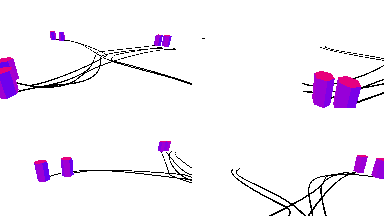
\includegraphics[width=134.71pt,height=75.77pt]{res_0001.png}};
%Shape: Rectangle [id:dp9113542083253017] 
\draw   (25.14,218.97) -- (204.75,218.97) -- (204.75,319.63) -- (25.14,319.63) -- cycle ;
%Straight Lines [id:da6295243822711887] 
\draw    (114.94,218.97) -- (114.94,319.63) ;
%Straight Lines [id:da13331215562102816] 
\draw    (24.75,269.3) -- (204.27,269.3) ;


%Image [id:dp4511992742946067] 
\draw (534.31,269.13) node  {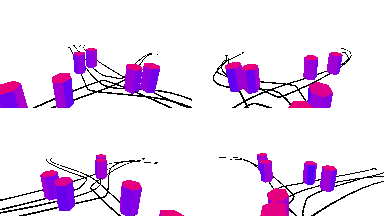
\includegraphics[width=133.76pt,height=75.24pt]{res_0040.png}};
%Shape: Rectangle [id:dp34987763791711735] 
\draw   (445.13,218.97) -- (623.73,218.97) -- (623.73,319.06) -- (445.13,319.06) -- cycle ;
%Straight Lines [id:da2902918967122481] 
\draw    (534.43,218.97) -- (534.43,319.06) ;
%Straight Lines [id:da16020670289119399] 
\draw    (444.75,269.01) -- (623.25,269.01) ;


%Image [id:dp8063348003256079] 
\draw (734.81,269.41) node  {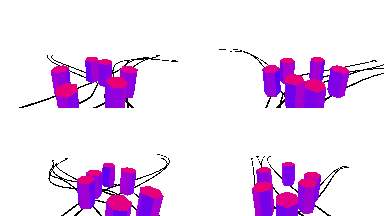
\includegraphics[width=134.5pt,height=75.66pt]{res_0060.png}};
%Shape: Rectangle [id:dp09591960950882639] 
\draw   (645.14,218.97) -- (824.75,218.97) -- (824.75,319.63) -- (645.14,319.63) -- cycle ;
%Straight Lines [id:da12607810159318578] 
\draw    (734.94,218.97) -- (734.94,319.63) ;
%Straight Lines [id:da01310243996367122] 
\draw    (644.75,269.3) -- (824.27,269.3) ;


%Image [id:dp3562017796779977] 
\draw (934.94,269.48) node  {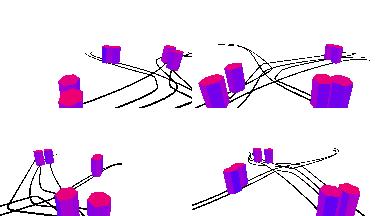
\includegraphics[width=134.71pt,height=75.77pt]{res_0080.png}};
%Shape: Rectangle [id:dp6762988492152433] 
\draw   (845.14,218.97) -- (1024.75,218.97) -- (1024.75,319.63) -- (845.14,319.63) -- cycle ;
%Straight Lines [id:da08080987030122322] 
\draw    (934.94,218.97) -- (934.94,319.63) ;
%Straight Lines [id:da642092361082927] 
\draw    (844.75,269.3) -- (1024.27,269.3) ;



% Text Node
\draw (713,175.4) node [anchor=north west][inner sep=0.75pt]    {$t\ =60$};
% Text Node
\draw (91.33,178.31) node [anchor=north west][inner sep=0.75pt]    {$t\ =\ 0$};
% Text Node
\draw (912.5,184.4) node [anchor=north west][inner sep=0.75pt]    {$t\ =80$};
% Text Node
\draw (512,181.4) node [anchor=north west][inner sep=0.75pt]    {$t\ =40$};
% Text Node
\draw (308.71,182.4) node [anchor=north west][inner sep=0.75pt]    {$t\ =20$};


\end{tikzpicture}

      }
      \caption{%
        Illustration of a view planning scenario taken
        from~\citep{hughes2024cdc}.
        Robots successfully track subjects despite pairs switching partners as
        they cross.
        \emph{Although this example features drones, the same methods are
        applicable to coordination of other sorts of camera platforms.}
      }%
      \label{fig:multi-robot-videography}
\end{figure*}

\begin{figure}
  \centering
  \begin{subfigure}{0.463\linewidth}
    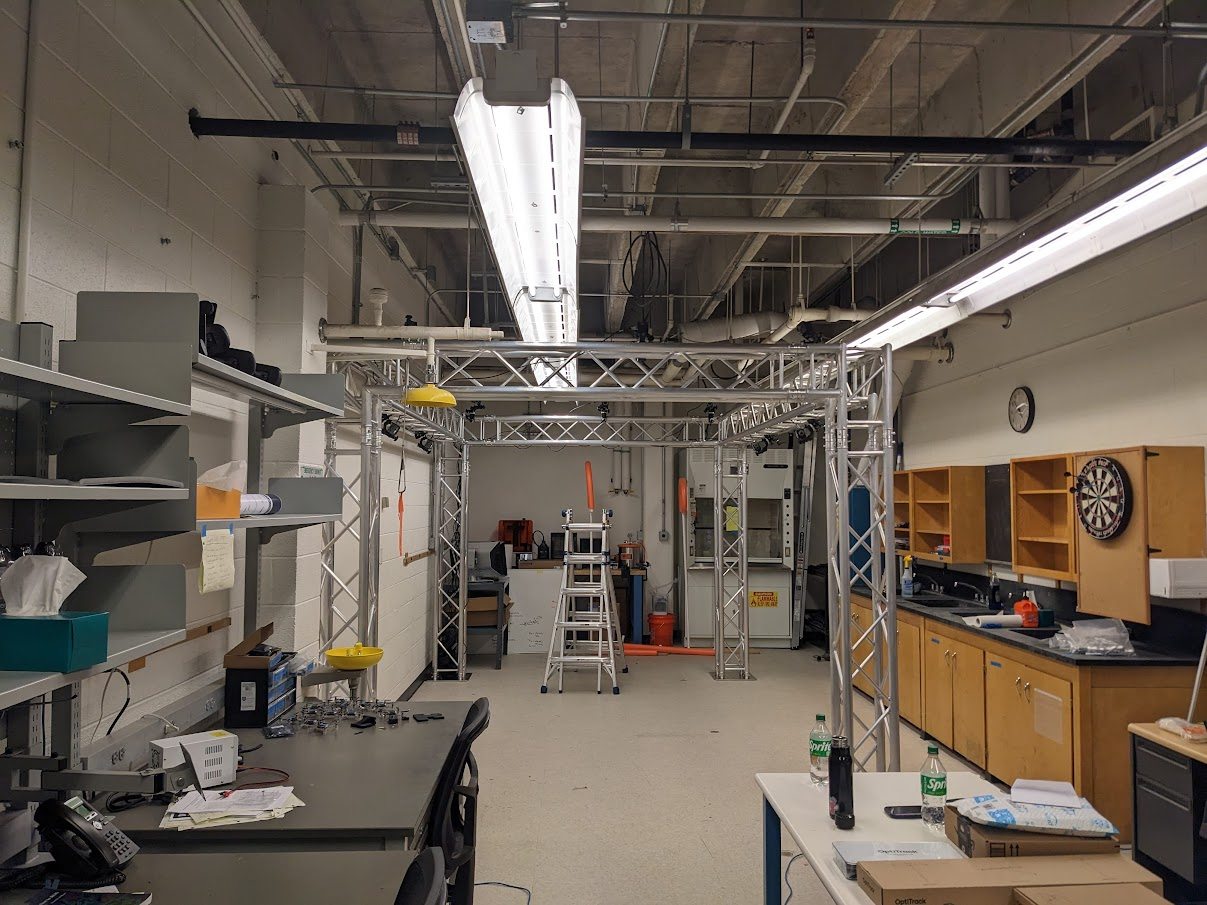
\includegraphics[width=\linewidth,trim={300 135 300 330},clip]{figures/flight_area}
    \caption{Motion capture system}%
    \label{subfig:motion_capture}
  \end{subfigure}
  \begin{subfigure}{0.50\linewidth}
    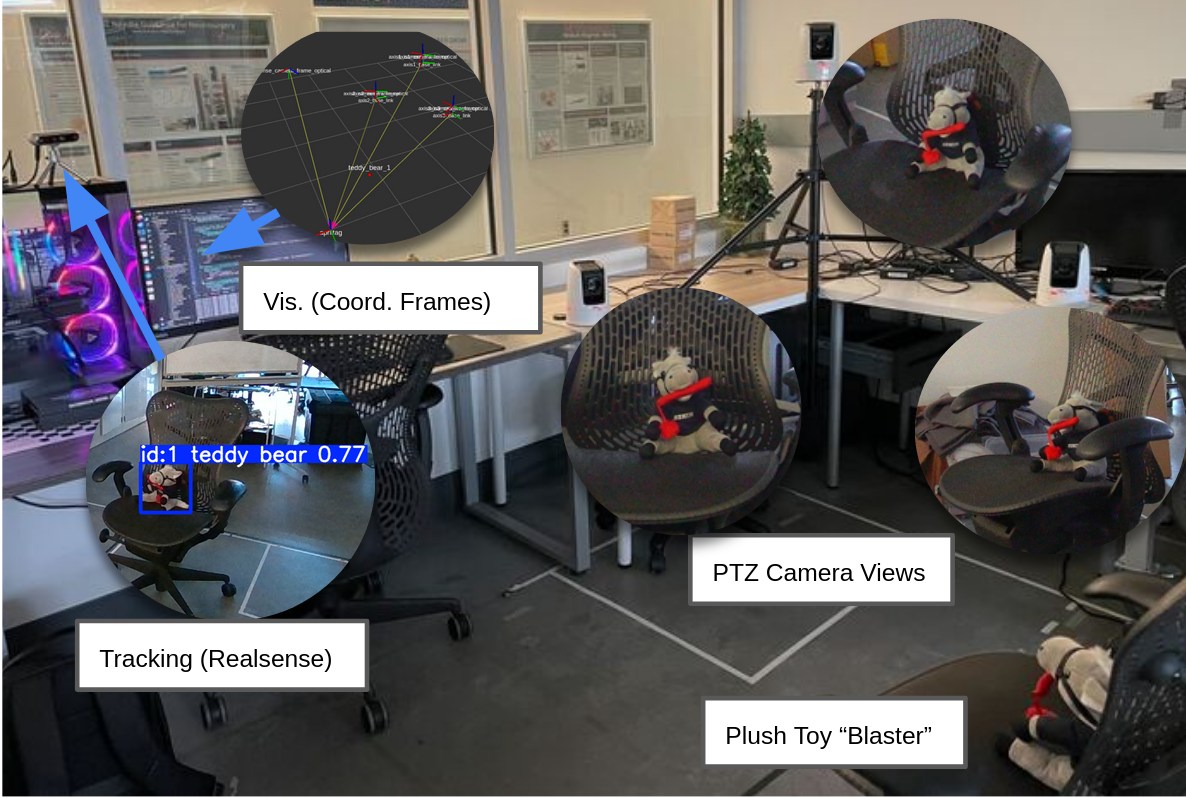
\includegraphics[width=\linewidth]{figures/PTZ_Videography_Full_System}
    \caption{PTZ videography system}%
    \label{subfig:videography}
  \end{subfigure}
  \caption{Systems and equipment:
    (\subref{subfig:motion_capture})
    Motion capture system and truss to be leverage for laboratory
    experiments.
    (\subref{subfig:videography})
    Illustration of videography system including
    object tracking via Realsense RGBD camera,
    three pan-tilt-zoom cameras filming a plush  toy of ``Blaster''
    (the Mines mascot),
    and computer visualization of 3D locations of cameras and the tracked
    subject.
  }
  \label{fig:hardware-systems}
\end{figure}

% Expected outcomes and results (separate tangible and intangible outcomes)
\section{Expected output \& innovation}

The specific outcomes of proposed work are as follows:
\begin{itemize}
  \item Publication of approach and experimental results in premier robotics
    conferences (IROS and ICRA)
  \item Demonstration of proof of concept pan-tilt-zoom markerless motion
    capture system capable of autonomously tracking and reconstructing multiple
    moving subjects
  \item Laboratory and field evaluation of above system
  \item Open source release of planner implementation and other software modules
    where appropriate
\end{itemize}
We expect that our work will spur increased interest in development of similar
low-cost, high-capture-volume motion capture methods.
The development of this technology will in turn reduce barriers to motion
capture data collection for sports, dance, and various performances.
This in turn will enable collection of novel datasets in these domains and
integration into practice, e.g. review of practice film.
Follow-on work may include development of methods for behavior prediction to
improve closed loop control performance or integration of methods for dense
reconstruction such based on Gaussian splatting.

\subsection{Future work and proposed extensions}

\micah{Future work is a bit all over the place. Revise and clean up.}

During the initial one-year timeline, our research efforts on markerless motion
capture will be limited to reconstruction of human skeletal pose.
If this project is extended for another year, we expect to focus on enabling
dense motion capture and reconstruction.
Methods for dense reconstruction of dynamic environments, e.g. methods for
dynamic Gaussian splatting~\citep{zheng2025cvpr} are quickly making dense
dynamic reconstruction more accessible.
However, current methods are often limited to laboratory environments and
additional instrumentation to compute accurate depth
measurements~\citep{zheng2025cvpr}.

We expect our activities would focus on developing sytems for dense
reconstruction and addressing subsequent challenges for planning and autonomy.
From a systems standpoint, achieving dense reconstruction with PTZ camera will
likely involve
extension of metric depth estimation models \citet{} suitable for cameras with
variable intrinsics and integrating with state-of-art tools for Gaussian
splatting~\citep{zheng2025cvpr}.
Moreover, we expect dense, dynamic reconstruction to exacerbate challenges
related to \emph{resolution} and \emph{coverage}.
At the same time, a strength of our approach is that because we model and
optimize pixel densities over the surface of the scene directly, our methods are
therefore suitable to incorporating these twin challenges into our design and
modeling.
In this sense, coverage and resolution are requirements---we can adapt our
planning approach accordingly and design camera systems (numbers, placements,
and models of cameras) to meet these requirements.

% Describe team composition
\section{Team and experience}

\noindent
Team composition:
\begin{itemize}
  \item PI: Prof. Micah Corah will supervise the proposed work.
  \item RA: One graduate student (MS or PhD) will be supported and will lead
    implementation of the technical approach
%  \item Undergrad RA(s): When appropriate, we will recruit and include
%    undergraduate researchers, especially to support subsystem development and
%    execution of laboratory and field experiments
  \item Academic integration: When appropriate, we will incorporate graduate and
    undergraduate student contributions
    (via independent study and the Mines Field Session\footnote{%
      Field Session:
      \url{https://www.mines.edu/oredigger-experience/field-session/}
    }and Capstone Design\footnote{%
      Capstone Design: \url{https://capstone.mines.edu/}
    } programs),
    especially to support subsystem development and
    execution of laboratory and field experiments
\end{itemize}

Prof. Micah Corah is an Assistant Professor of Computer Science at the Colorado
School of Mines where directs the
Navigation, Aerial-robots, and Perception Planning Lab (NAPPLab)\footnote{%
  NAPPLab: \url{https://www.napplab.org/}
}
Micah has extensive experience in the area of active perception and especially
regarding optimization for coordination of multiple
cameras~\citep{corah2019auro,corah2018cdc,corah2021iros}.
Recently, Micah has become interested in applying such methods to tasks that
involve filming multiple moving subjects (athletes, performers) from multiple
perspectives~\citep{suresh2024iros,hughes2024cdc}.
These contributions of these works form the basis for this proposal.

Micah's work is also representative of interest in the relationship between
representations of three-dimensional environments and coordinating camera
motions to produce such representations, especially via the process of robot
exploration or autonomous
mapping~\citep{corah2019ral,corah2021icra,corah2019auro,goel2019fsr,kim2023ral}
In particular, this interest led to contributions toward Gaussian mixture
mapping~\citep{corah2019ral} preceding the advent and popularity of Gaussian
splatting methods for reconstruction.

Micah also has a background in development and deployment of robotic mobility
and camera systems.
As a postdoctoral researcher at the Jet Propulsion Laboratory, Micah competed
with team CoSTAR in the final stage of the DARPA Subterranean
Challenge~\citep{morrell2024addendum}.
This competition involved field deployment of multi-robot teams to search and
explore underground environments representative of caves, mines, and urban
underground.
Micah's contributions to team CoSTAR are also representative in a longstanding
interest in development robot autonomous perceptions---especially single- and
multi-robot drone systems for exploration of
three-dimensional environments~\citep{corah2019auro,kim2023ral,goel2019fsr}.
Micah will draw on his experience in development of robotic perception systems
and regarding logistics for robot field deployments while supervising the
proposed work.

% Fakesection: Bibliography
\bibliographystyle{plainnat}
\setlength{\bibsep}{4pt plus 0.3ex}
\bibliography{publisher_abbreviations,micah_corah_papers,markerless_refs,bibliography}

\newpage
\section{Budget}

The budget for the proposed work is listed in Table.~\ref{tab:budget}.


\begin{table}[!htb]
\centering
\begin{tabular}{|l|r|}
\hline
\multicolumn{1}{|c|}{Item}        & \multicolumn{1}{c|}{Amount in USD} \\ \hline
PI Corah (15 days)                & 10,001                      \\ \hline
Fringe                            & 3,420                       \\ \hline
Ph.D. Student Stipend (1 Year)
                                  & 40,000                      \\ \hline
Ph.D. Student Tuition             & 31,195                      \\ \hline
Undergrad. Research Asst.         & 5,000                       \\ \hline
\textbf{Subtotal--Salary}         & 55,001                      \\ \hline
\textbf{Subtotal--Fringe}         & 34,615                      \\ \hline
\textbf{Total Personnel Costs}    & 89,616                      \\ \hline
                                  &                             \\ \hline
Capital Equipment                 & 10,000                      \\ \hline
Travel                            & 7,045                       \\ \hline
Materials \& Supplies             & 1,000                       \\ \hline
                                  &                             \\ \hline
\textbf{Total Direct Costs}       & 107,661                     \\ \hline
                                  &                             \\ \hline
\textbf{Modified Total Direct
        Costs (MTDC)}             & 66,466                      \\ \hline
\textbf{Indirect Cots (63.7\%
        applied to MTDC)}         & 42,339                      \\ \hline
                                  &                             \\ \hline
\textbf{Total Sponsor Costs}      & 149,999                     \\ \hline
\end{tabular}
\caption{Budget.}
\label{tab:budget}
\end{table}


\end{document}
